\documentclass[oneside,a4paper,12pt]{article}

\usepackage{setspace}
\usepackage{listings}
\usepackage{pdfpages}
\usepackage{graphicx,subfigure,wrapfig}
\usepackage{multirow}
\usepackage{multicol}
\usepackage[a4paper,margin=2.5cm]{geometry}
\usepackage{amsmath,amssymb}
\usepackage{array}
\usepackage{float}
\usepackage{booktabs}
\usepackage{xcolor}
\usepackage[bottom]{footmisc}
\usepackage[colorlinks,linkcolor=blue,citecolor=blue]{hyperref}
\usepackage{xepersian}

\geometry{margin=1in,bottom=1.1in,footskip=.4in}
\renewcommand{\baselinestretch}{1.4}
\linespread{1.6}
\setlength{\parskip}{0.45em}

\settextfont[
    Path=fonts/,
    Extension=.ttf,
    BoldFont=B-Nazanin-Bold
]{B-Nazanin}

\setlatintextfont[
    Extension=.otf,
    BoldFont=lmroman10-bold,
    ItalicFont=lmroman10-italic
]{lmroman10-regular}

\definecolor{codebg}{RGB}{247,247,247}
\definecolor{codeframe}{RGB}{210,210,210}
\definecolor{codecomment}{RGB}{70,120,70}
\definecolor{codekeyword}{RGB}{30,70,150}
\definecolor{BrickRed}{RGB}{181,72,93}

\lstdefinelanguage{Go}{
  morekeywords={break,default,func,interface,select,case,defer,go,map,struct,chan,else,goto,package,switch,const,fallthrough,if,range,type,continue,for,import,return,var},
  sensitive=true,
  morecomment=[l]{//},
  morecomment=[s]{/*}{*/},
  morestring=[b]",
  morestring=[b]'
}

\lstset{
  language=Go,
  basicstyle=\ttfamily\small,
  keywordstyle=\color{codekeyword}\bfseries,
  commentstyle=\color{codecomment},
  stringstyle=\color{BrickRed},
  backgroundcolor=\color{codebg},
  frame=single,
  rulecolor=\color{codeframe},
  breaklines=true,
  columns=fullflexible,
  keepspaces=true,
  showstringspaces=false,
  numbers=left,
  numberstyle=\tiny\color{gray},
  xleftmargin=1.8em,
  framexleftmargin=1.4em,
  captionpos=b
}

\setlength{\emergencystretch}{3em}
\renewcommand{\labelitemi}{\ensuremath{\bullet}}

\newcommand{\مهم}[1]{\textbf{#1}}
\newcommand{\Arch}[1]{\lr{\texttt{#1}}}
\newcommand{\درصد}[1]{\lr{#1\%}}

\begin{document}

% ==================== صفحه عنوان ====================

\pagestyle{empty}

\begin{center}


\includegraphics[scale=0.2]{images/logo.png}

\vspace{-0.2cm}
دانشگاه صنعتی شریف\\[-0.3em]
دانشکده مهندسی کامپیوتر

\begin{large}
\vspace{0.5cm}
\end{large}

\vspace{1.5cm}

عنوان:\\[1.2em]
{\LARGE\textbf{تحلیل نقص‌های برخورد و طراحی حافظه نهان قربانی}}

\vspace{1cm}

{\Large\textbf{\lr{Conflict Miss Analysis and Victim Cache Design}}}

\vspace{2cm}

اعضای گروه\\[0.5em]
{\large\textbf{
علی فتحی\\
محمدپارسا محمودآبادی آرانی\\
محمدمهدی مرادی
}}

\vspace{0.7cm}

نام درس\\[0.5em]
{\large\textbf{معماری کامپیوتر}}

\vspace{0.7cm}

{\large\textbf{نیم‌سال تحصیلی ۱۴۰۴۲}}

نام استاد درس\\[0.5em]
{\large\textbf{دکتر حمید سربازی آزاد}}

\vspace{1.2cm}

\end{center}

\newpage

% ==================== محتوای گزارش ====================

\pagestyle{plain}
\pagenumbering{arabic}

\tableofcontents
\listoffigures
\clearpage
\listoftables
\clearpage

\noindent \مهم{چکیده}: هدف این پروژه بررسی افت کارایی ناشی از نقص‌های برخورد در حافظه نهان مستقیم‌نگاشت و ارزیابی حافظه نهان قربانی به‌عنوان راه‌حل این مسئله است. ابتدا رفتار معماری پایه شامل حافظه نهان سطح اول، حافظه نهان سطح دوم و حافظه اصلی در شبیه‌ساز رویدادمحور آکیتا مدل‌سازی شد. سپس با یک برنامه محک هدفمند، آدرس‌هایی تولید شدند که پیوسته به یک خط سطح اول نگاشت می‌شوند تا اخراج‌های تکراری، افزایش مراجعه به سطح دوم و هزینه زمانی نقص برخورد به‌روشنی مشاهده شود.

در معماری پیشنهادی، یک حافظه قربانی هشت‌مدخلی و تمام‌انجمنی میان دو سطح حافظه نهان قرار گرفت. بلوک اخراج‌شده از سطح اول ابتدا در این حافظه نگهداری می‌شود و در صورت مراجعه دوباره، با بلوک فعلی سطح اول به‌صورت اتمیک جابه‌جا می‌گردد. برای مدیریت ظرفیت محدود نیز دو سیاست \lr{FIFO} و \lr{LRU} پیاده‌سازی و مقایسه شدند. ارزیابی بر پایه تعداد اصابت و عدم اصابت، ترافیک سطح دوم، تعداد جابه‌جایی‌ها، زمان کل اجرا و میانگین زمان دسترسی انجام شده است.

نتایج نشان می‌دهد که در برنامه محک برخوردی، افزودن حافظه قربانی تعداد خواندن‌های سطح دوم را از ۳۲ به ۴ و میانگین زمان دسترسی را از \lr{25.5} به ۱۷ چرخه کاهش می‌دهد. در الگوی ترکیبی نیز سیاست \lr{LRU} با حفظ بلوک‌های پراستفاده، ۱۲۸ اصابت بیشتر از \lr{FIFO} ایجاد می‌کند و زمان اجرا را ۱۵۳۶ چرخه کاهش می‌دهد. بنابراین حافظه قربانی در الگوهای برخوردی می‌تواند با هزینه سخت‌افزاری اندک، ترافیک سطوح پایین‌تر و زمان دسترسی را به‌طور محسوسی کاهش دهد؛ بااین‌حال میزان سود آن به الگوی دسترسی و سیاست جایگزینی وابسته است.

\section{صورت مسئله و هدف پروژه}

\subsection{مسئله نقص برخورد}

در حافظه نهان مستقیم‌نگاشت، هر بلوک حافظه اصلی فقط در یک خط مشخص قرار می‌گیرد. اگر چند بلوک پرکاربرد اندیس یکسانی داشته باشند، پی‌درپی یکدیگر را اخراج می‌کنند؛ حتی زمانی که بخش دیگری از حافظه نهان خالی است. این وضعیت \مهم{نقص برخورد} نام دارد و با افزایش مراجعه به سطوح پایین‌تر، ترافیک حافظه و زمان اجرا را بیشتر می‌کند. هدف پروژه، کاهش این هزینه با افزودن یک حافظه نهان قربانی کوچک و مقایسه دو سیاست جایگزینی \lr{FIFO} و \lr{LRU} است.

در پیکربندی این پروژه، حافظه نهان \lr{L1} دارای ظرفیت ۴ کیبی‌بایت، اندازه بلوک ۶۴ بایت و درجه انجمنی یک است؛ بنابراین ۶۴ خط دارد. اندیس یک بلوک با رابطه زیر محاسبه می‌شود:

\begin{equation}
\mathrm{L1Index}=\mathrm{BlockAddress}\bmod 64.
\end{equation}

بنابراین بلوک‌هایی که شماره آن‌ها ۶۴ واحد با هم فاصله دارد، به یک خط \lr{L1} نگاشت می‌شوند. برنامه محک \Arch{conflict} با تولید آدرس‌هایی به فاصله کل ظرفیت \lr{L1} همین وضعیت را ایجاد می‌کند.

\subsection{راه‌حل حافظه نهان قربانی}

حافظه نهان قربانی یک بافر کوچک تمام‌انجمنی میان \lr{L1} و \lr{L2} است. بلوک اخراج‌شده از \lr{L1} ابتدا در این بافر قرار می‌گیرد. در عدم اصابت بعدی \lr{L1}، اگر بلوک درخواستی در حافظه قربانی باشد، با بلوک فعلی خط متناظر جابه‌جا می‌شود و نیازی به خواندن از \lr{L2} نخواهد بود.

حافظه قربانی هشت مدخل دارد و از دو سیاست جایگزینی پشتیبانی می‌کند:

\begin{itemize}
\item \lr{FIFO}: بلوکی اخراج می‌شود که زودتر از همه وارد حافظه قربانی شده است؛ معیار تصمیم فیلد \lr{Inserted} است.
\item \lr{LRU}: بلوکی با قدیمی‌ترین زمان استفاده اخراج می‌شود؛ معیار تصمیم فیلد \lr{LastUsed} است. این مقدار هنگام خروج بلوک از \lr{L1} حفظ می‌شود.
\end{itemize}

\subsection{دامنه ارزیابی}

تحلیل کمّی روی سه توپولوژی زیر انجام شده است:

\begin{itemize}
\item \Arch{l1-l2}: معماری پایه شامل \lr{CPU $\rightarrow$ L1 $\rightarrow$ L2 $\rightarrow$ Main Memory}، بدون حافظه قربانی؛
\item \Arch{full-fifo}: معماری کامل با حافظه قربانی هشت‌مدخلی و سیاست \lr{FIFO}؛
\item \Arch{full-lru}: معماری کامل با حافظه قربانی هشت‌مدخلی و سیاست \lr{LRU}.
\end{itemize}

همه الگوهای دسترسی در این گزارش فقط درخواست خواندن تولید می‌کنند؛ ازاین‌رو مقدار \lr{L2 writes} در نتایج صفر است. مدل از درخواست نوشتن و بیت \lr{Dirty} نیز پشتیبانی می‌کند، اما ارزیابی جداگانه سیاست نوشتن در دامنه این پروژه قرار ندارد.

\section{طراحی معماری و اجرای رویدادمحور با آکیتا}

\subsection{پیکربندی سلسله‌مراتب حافظه}

جدول \ref{tab:config} پارامترهای مشترک سه توپولوژی ارزیابی‌شده را نشان می‌دهد. ثابت بودن این پارامترها باعث می‌شود تنها اثر افزودن حافظه قربانی و سیاست جایگزینی آن اندازه‌گیری شود.

\begin{table}[H]
\centering
\caption{پارامترهای پیش‌فرض سلسله‌مراتب حافظه}
\label{tab:config}
\begin{tabular}{p{5.3cm}p{4.2cm}p{4cm}}
\toprule
\textbf{مولفه} & \textbf{پیکربندی} & \textbf{تأخیر} \\
\midrule
\lr{L1 Cache} & ۴ کیبی‌بایت، ۶۴ بایت در هر بلوک، مستقیم‌نگاشت، ۶۴ خط & ۱ چرخه \\
\lr{Victim Cache} & ۸ مدخل، تمام‌انجمنی، \lr{FIFO/LRU} & ۲ چرخه \\
\lr{L2 Cache} & ۶۴ کیبی‌بایت، ۸-راهه، ۱۲۸ مجموعه، جایگزینی \lr{FIFO} & ۱۲ چرخه \\
حافظه اصلی & مدل بلوکی با آدرس بلوک & ۱۰۰ چرخه \\
اندازه کلمه در الگوی ترتیبی & ۴ بایت؛ ۱۶ کلمه در هر بلوک ۶۴ بایتی & فاقد تأخیر مستقل \\
\bottomrule
\end{tabular}
\end{table}

\subsection{ساختارهای داده اصلی}

برای جلوگیری از ناسازگاری میان سطوح حافظه، همه مولفه‌ها از مدل‌های مشترک استفاده می‌کنند:

\begin{itemize}
\item \lr{Request}: شناسه درخواست، آدرس بایتی، نوع عملیات خواندن یا نوشتن و اندازه دسترسی؛
\item \lr{Response}: شناسه درخواست، محل پاسخ‌گویی شامل \lr{L1}، حافظه قربانی، \lr{L2} یا حافظه اصلی، و تعداد چرخه‌های صرف‌شده؛
\item \lr{Block}: آدرس بلوک، برچسب، بیت‌های \lr{Valid} و \lr{Dirty}، زمان آخرین استفاده و زمان ورود.
\end{itemize}

آدرس ذخیره‌شده در \lr{Block}، آدرس بلوک است و از تقسیم آدرس بایتی بر اندازه بلوک به دست می‌آید. هر سطح حافظه اندیس و برچسب خود را از همین مقدار مشترک محاسبه می‌کند.

\subsection{ماشین حالت معماری پایه}

در توپولوژی \Arch{l1-l2}، هر درخواست ابتدا در \lr{L1} بررسی می‌شود. اصابت \lr{L1} بلافاصله پاسخ داده می‌شود. در عدم اصابت، شمارنده خواندن \lr{L2} افزایش یافته و \lr{L2} جست‌وجو می‌شود. اصابت \lr{L2} باعث نصب بلوک در \lr{L1} می‌شود؛ در غیر این صورت بلوک از حافظه اصلی خوانده، در \lr{L2} و سپس \lr{L1} نصب می‌شود. اگر نصب در \lr{L1} بلوکی را اخراج کند، آن بلوک مستقیماً به \lr{L2} فرستاده می‌شود.

\begin{figure}[H]
\centering
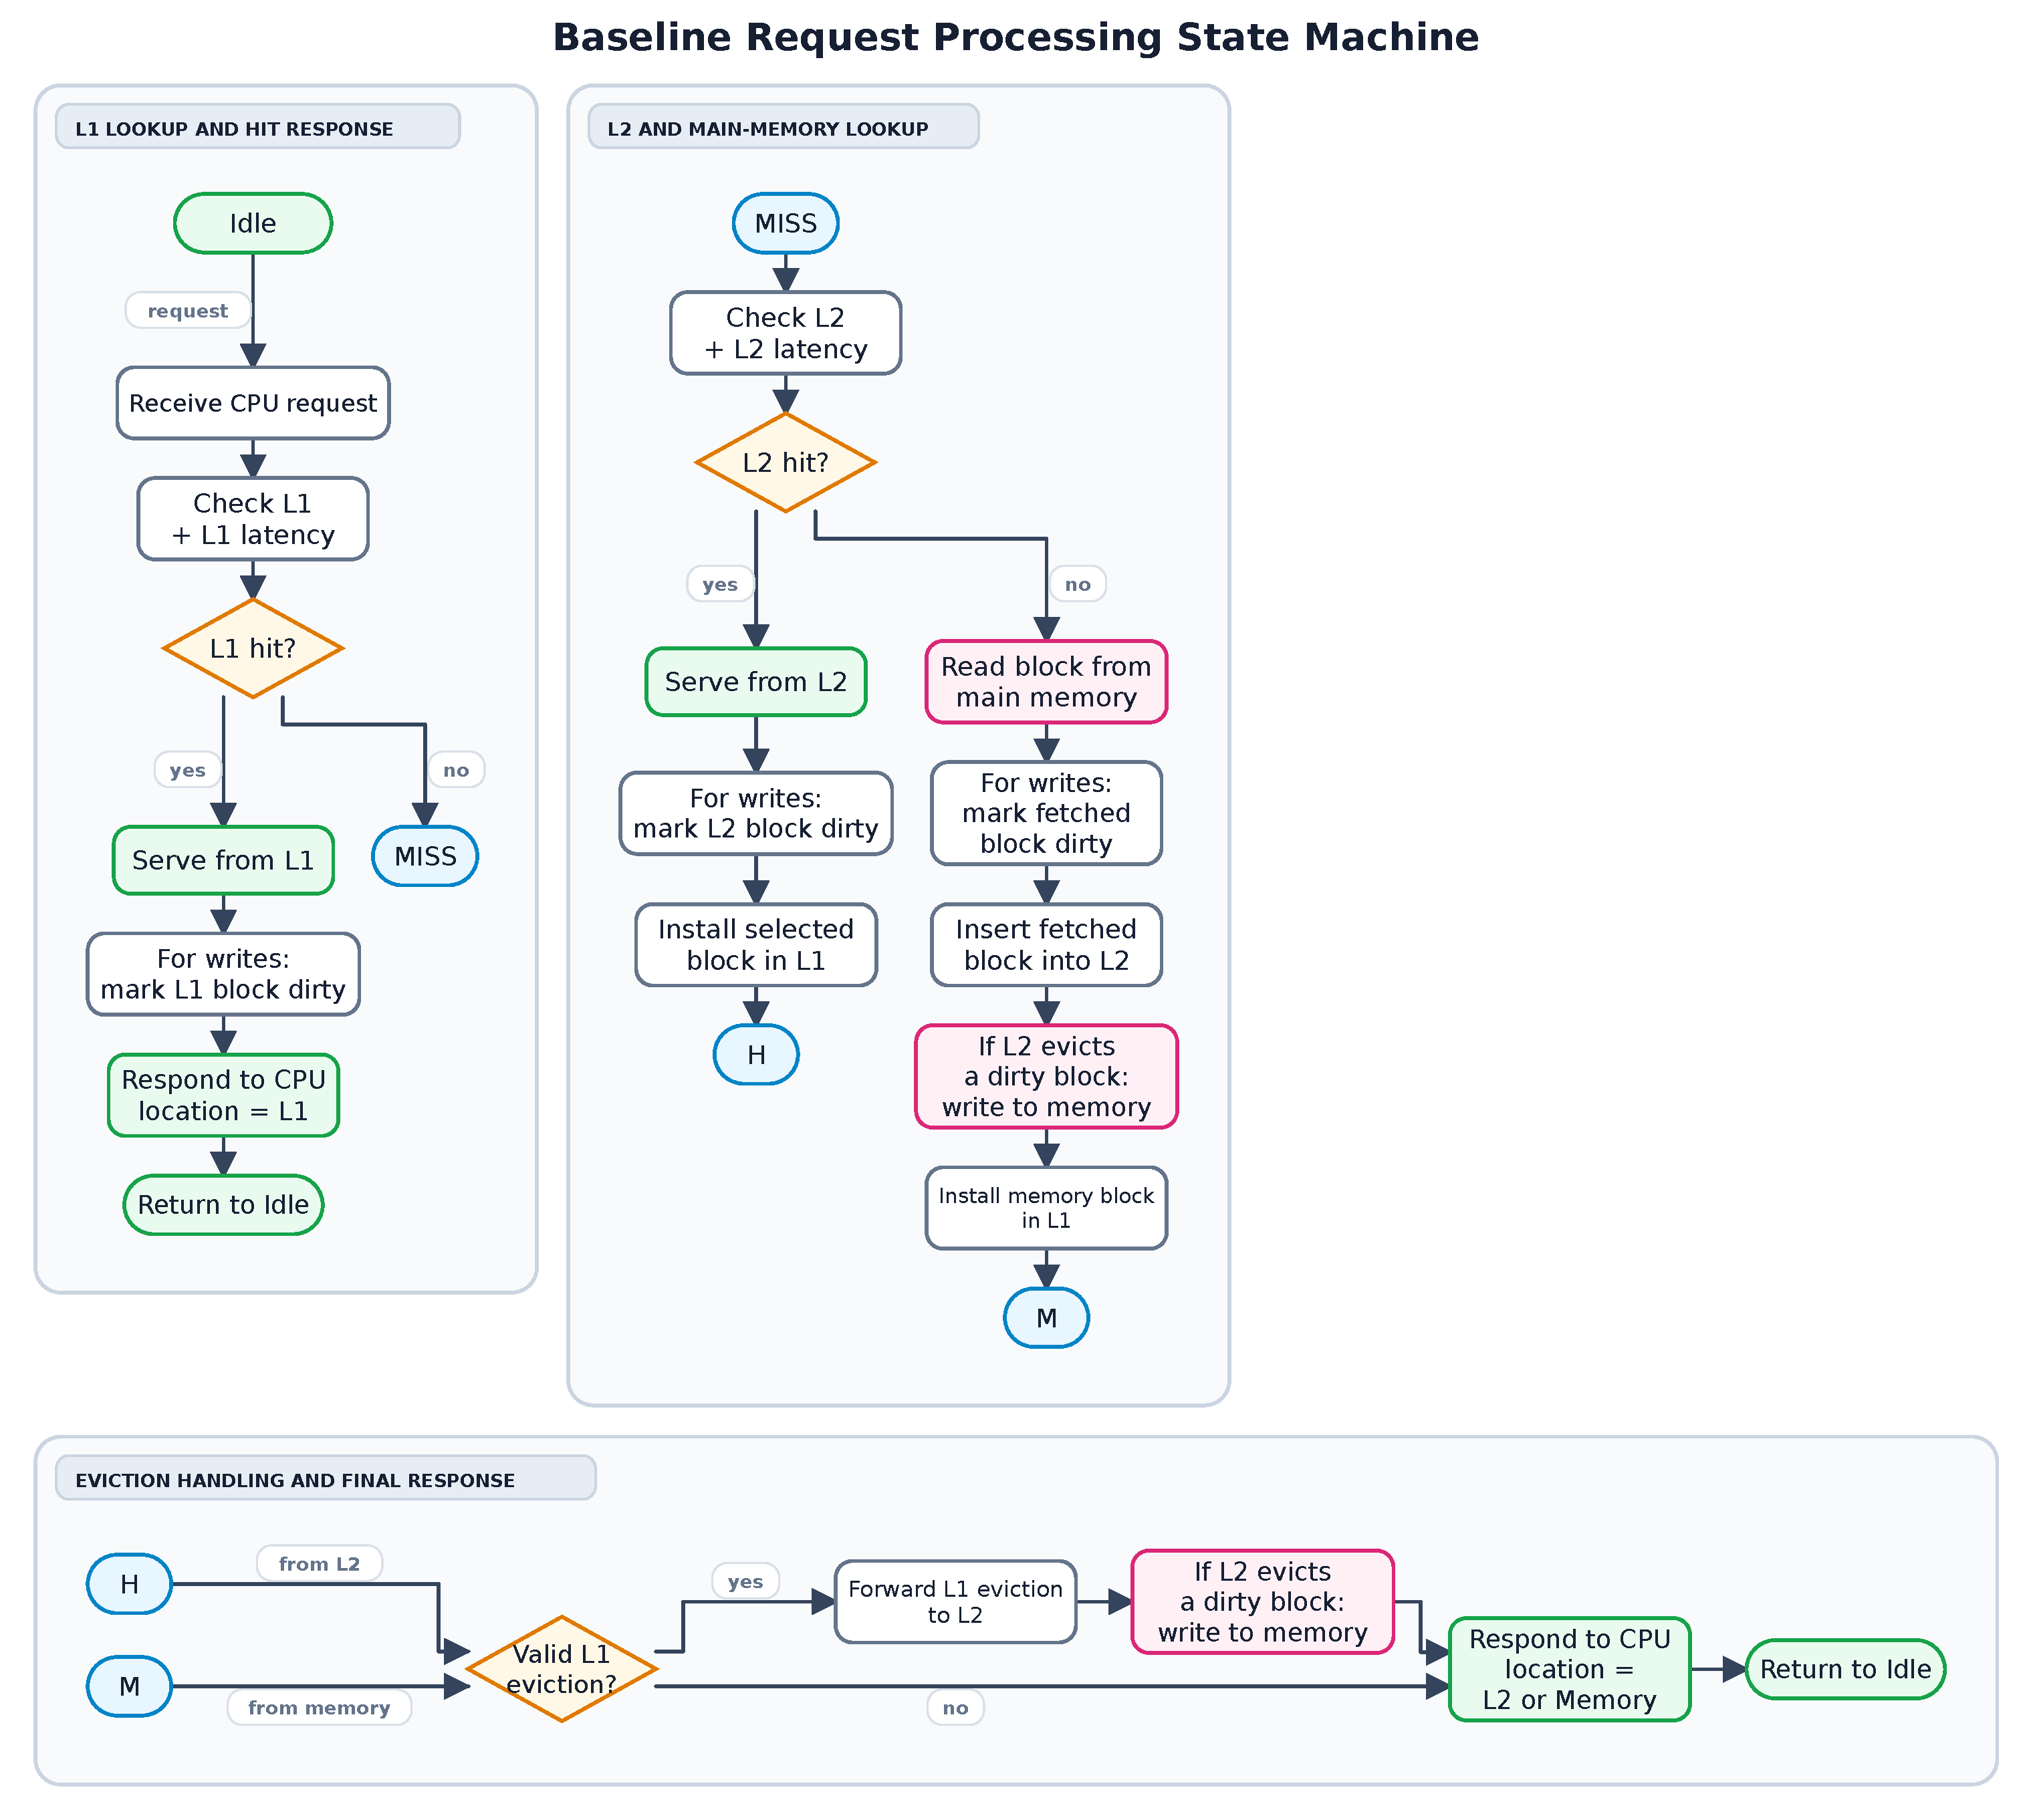
\includegraphics[width=.98\textwidth,height=.72\textheight,keepaspectratio]{images/01-baseline-request-fsm.pdf}
\caption{ماشین حالت پردازش درخواست در معماری پایه \Arch{l1-l2}}
\label{fig:baseline-fsm}
\end{figure}

\subsection{ماشین حالت معماری دارای حافظه قربانی}

در توپولوژی کامل، مرحله بررسی حافظه قربانی بین \lr{L1} و \lr{L2} افزوده می‌شود. اگر \lr{L1} دچار عدم اصابت و حافظه قربانی دارای بلوک درخواستی باشد، مسیر به حالت \lr{Victim Hit/Swap} می‌رود و هیچ درخواست خواندنی به \lr{L2} ارسال نمی‌شود. تنها در صورت عدم اصابت حافظه قربانی، \lr{L2} بررسی می‌شود. همچنین بلوک اخراجی از \lr{L1} ابتدا وارد حافظه قربانی می‌شود و فقط سرریز حافظه قربانی به \lr{L2} می‌رود.

\begin{figure}[H]
\centering
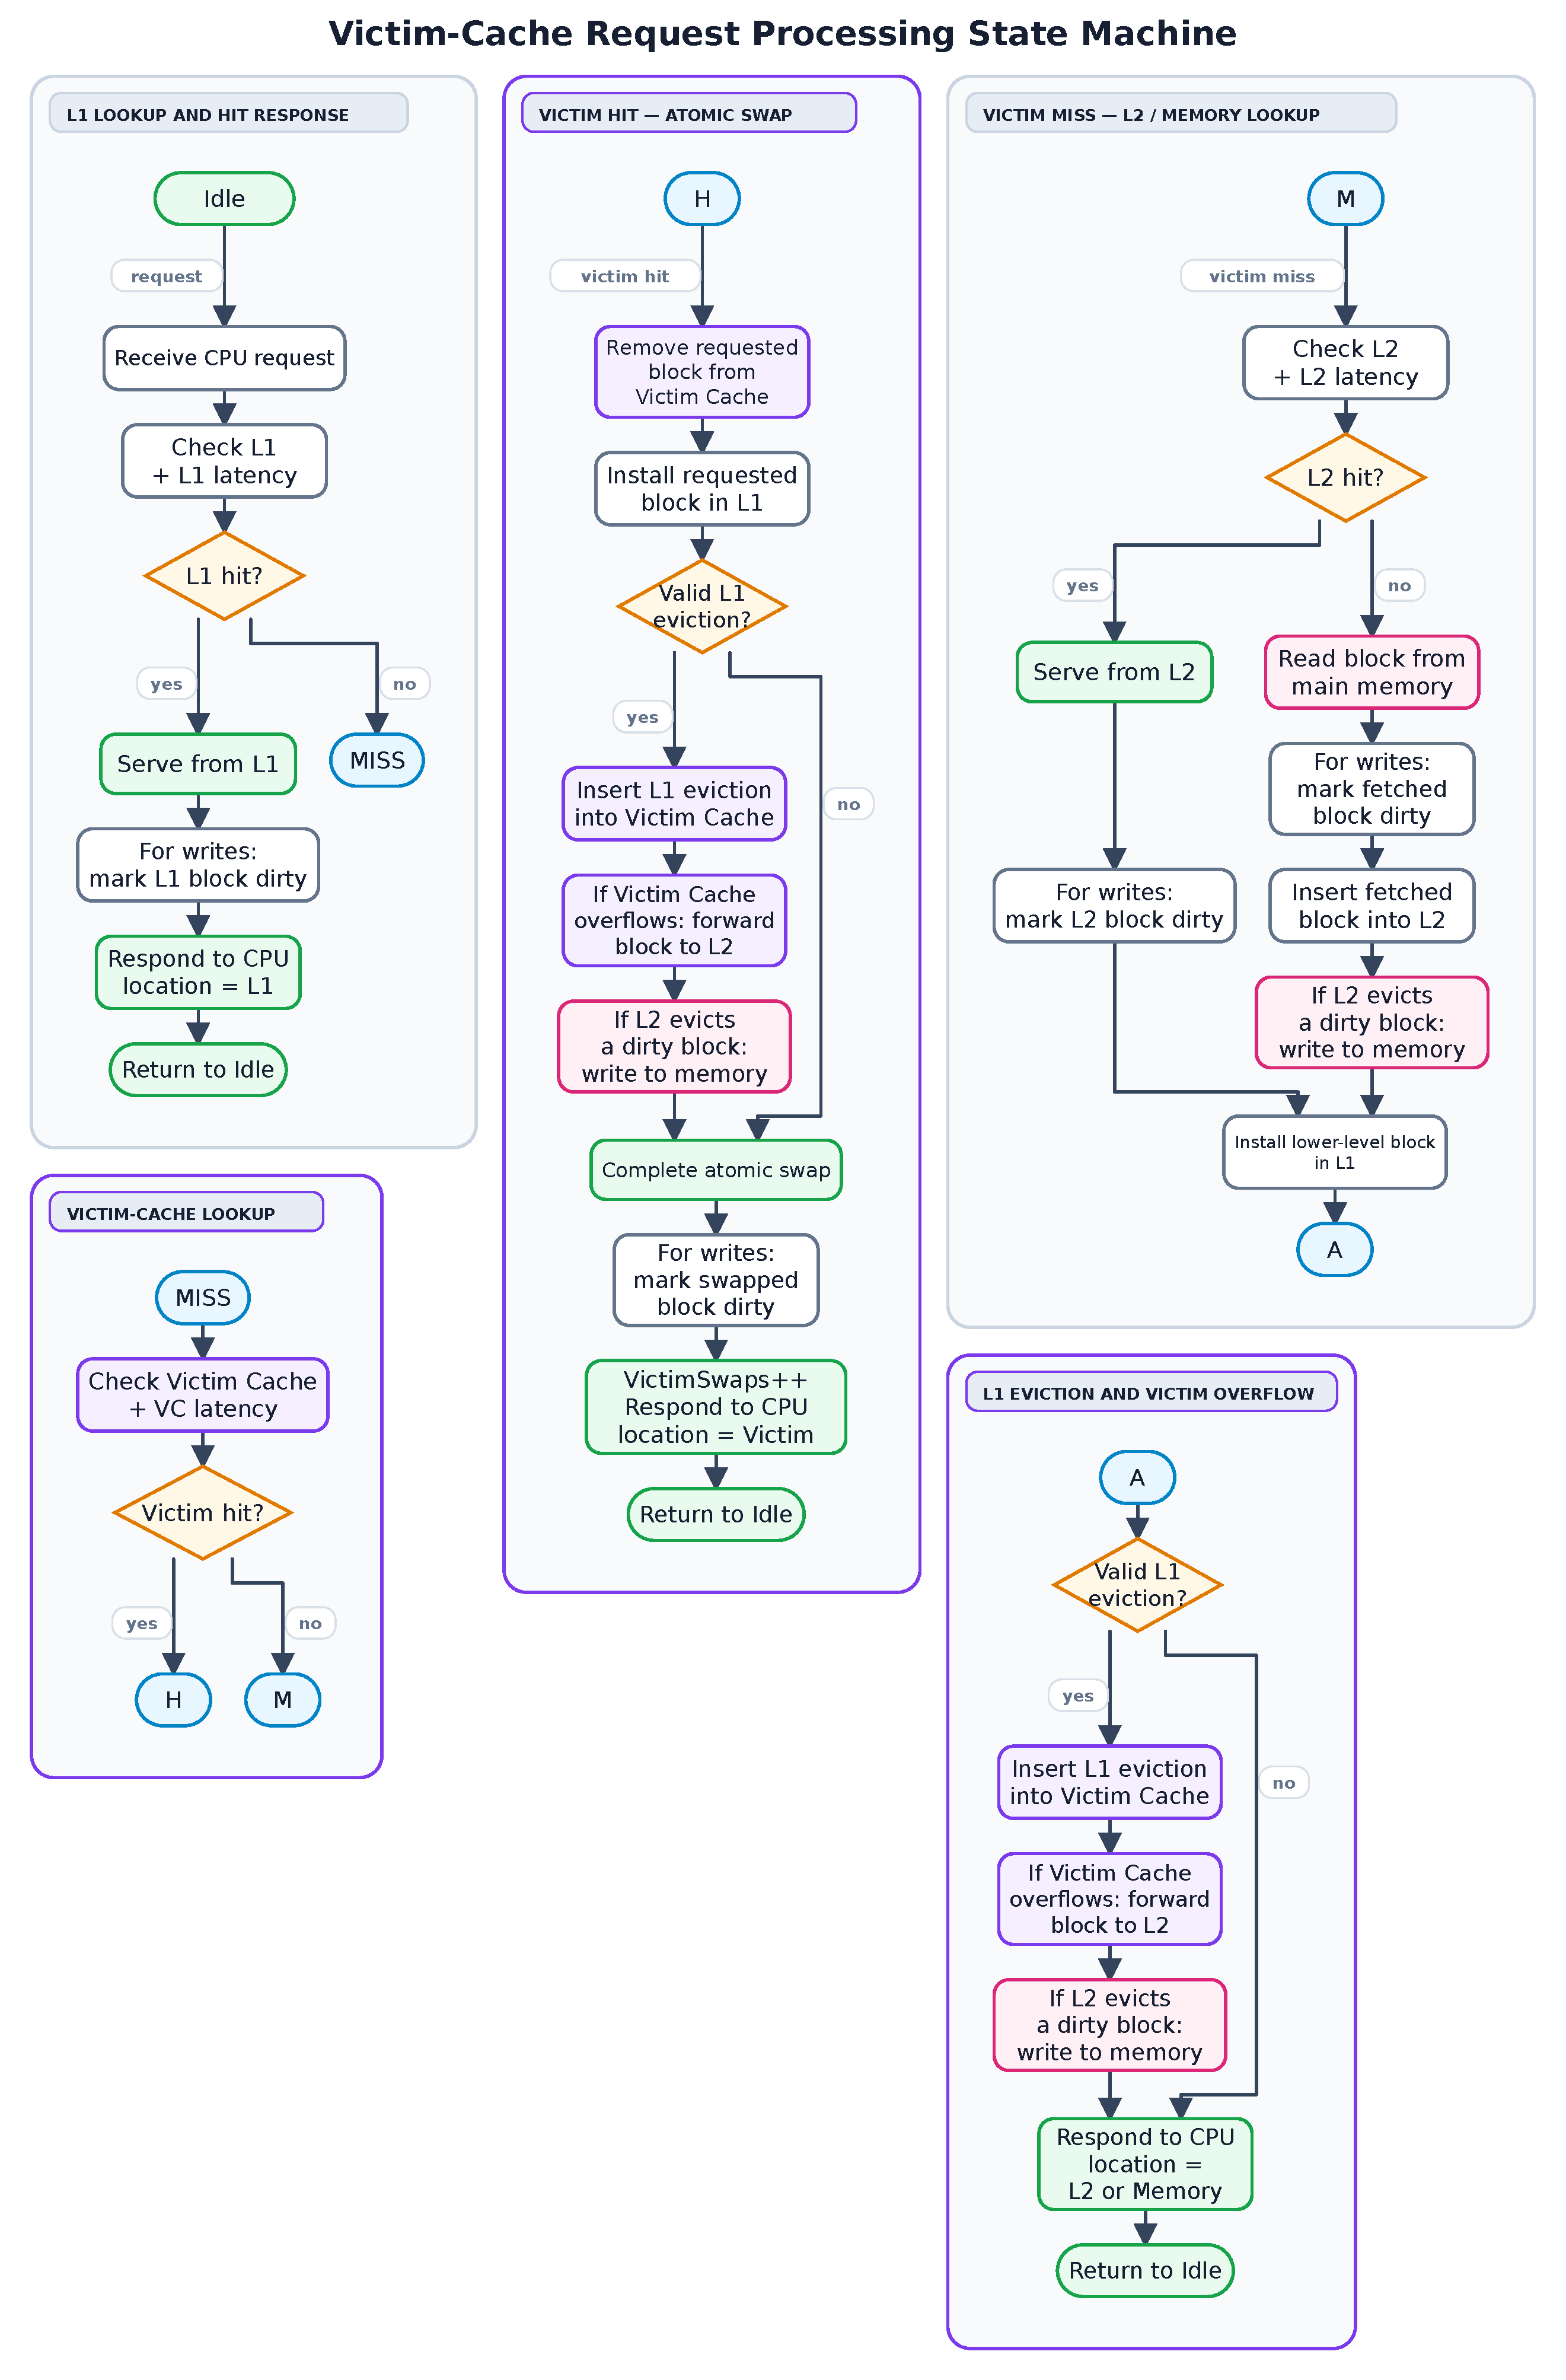
\includegraphics[width=.98\textwidth,height=.84\textheight,keepaspectratio]{images/02-victim-cache-request-fsm.pdf}
\caption{ماشین حالت پردازش درخواست در معماری کامل دارای حافظه قربانی}
\label{fig:victim-fsm}
\end{figure}

\subsection{توالی منطقی عملیات داخلی سلسله‌مراتب}

شکل \ref{fig:baseline-seq} ترتیب منطقی عملیات داخل یک فراخوانی \lr{System.Access} را در عدم اصابت کامل معماری پایه نشان می‌دهد. پیکان‌های این شکل نشان‌دهنده فراخوانی‌های درون‌سیستمی میان هماهنگ‌کننده و سطوح مختلف حافظه است که پس از دریافت درخواست، در داخل مولفه اجراکننده انجام می‌شوند.

\begin{figure}[H]
\centering
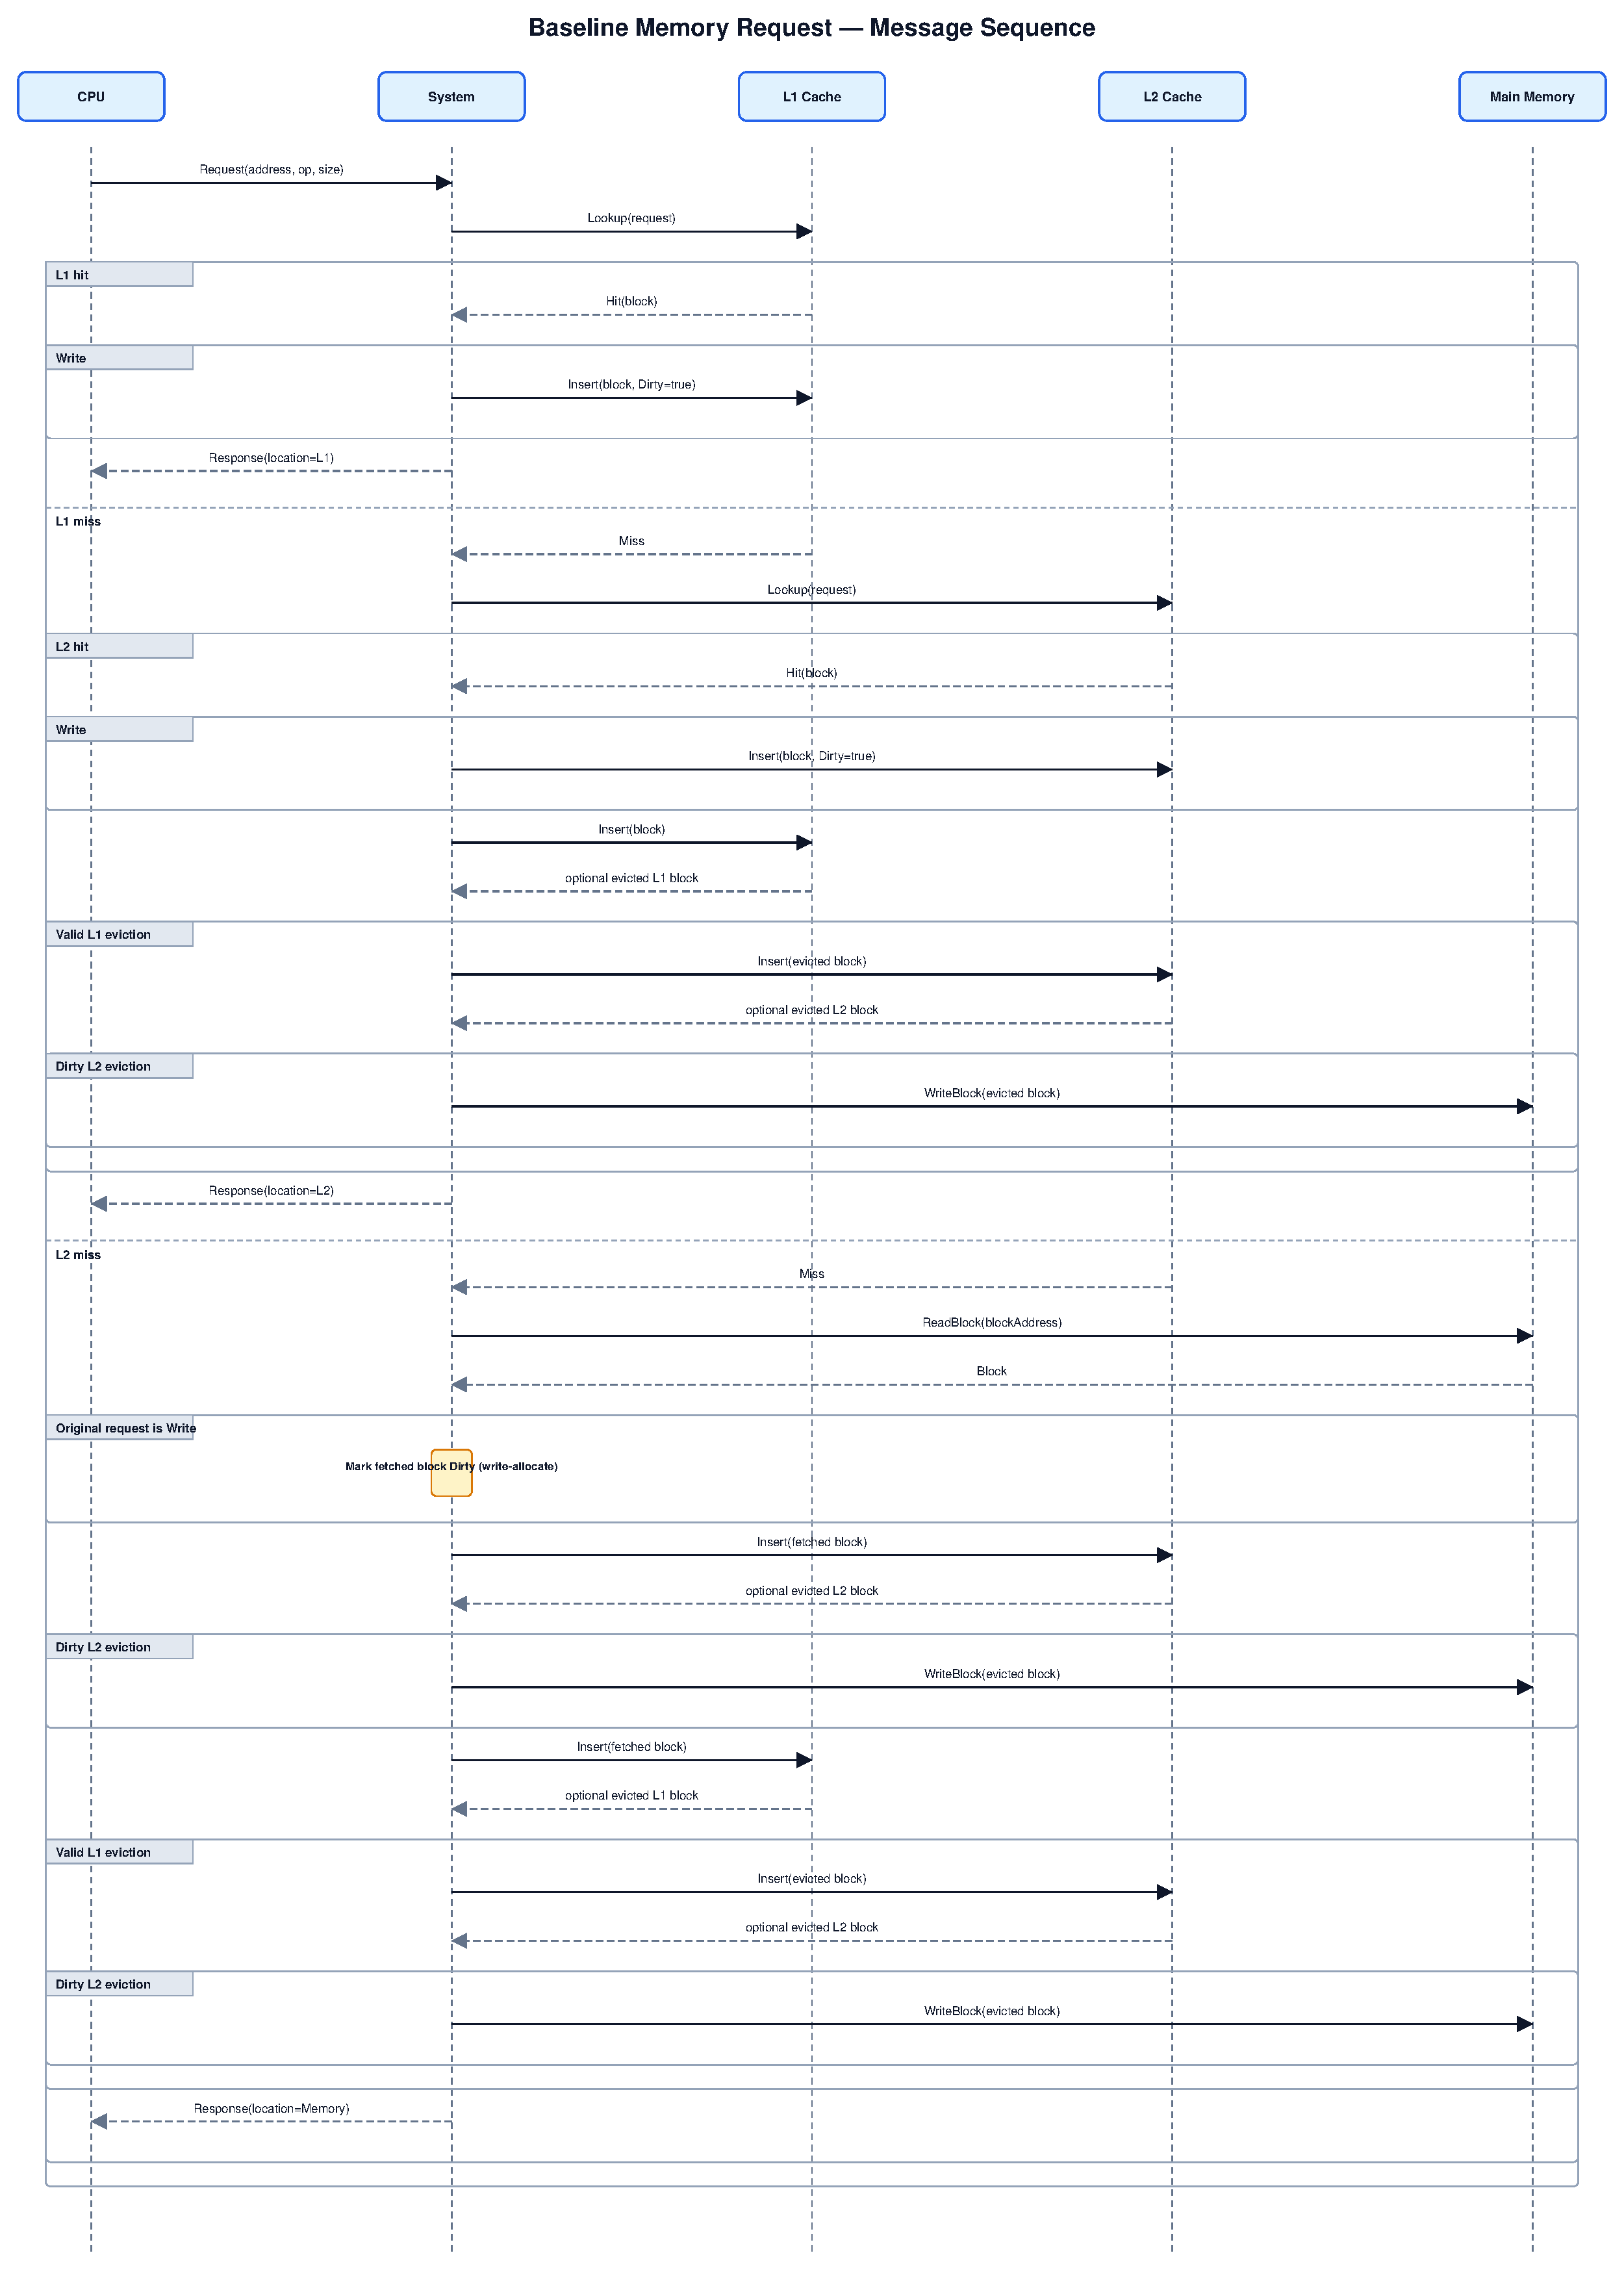
\includegraphics[width=.95\textwidth,height=.72\textheight,keepaspectratio]{images/06-baseline-message-sequence.pdf}
\caption{توالی منطقی عملیات \lr{System.Access} در معماری پایه برای مسیر عدم اصابت تا حافظه اصلی}
\label{fig:baseline-seq}
\end{figure}

شکل \ref{fig:victim-swap-seq} عملیات داخلی اصابت حافظه قربانی را نشان می‌دهد. بلوک درخواستی از حافظه قربانی حذف، در \lr{L1} نصب و بلوک اخراجی همان خط در مدخل خالی‌شده قرار داده می‌شود. پس از بازگشت \lr{System.Access}، مولفه اجراکننده آکیتا پاسخ را بلافاصله ارسال نمی‌کند؛ ابتدا یک \lr{completeAccessEvent} در زمان متناظر با تأخیر پاسخ زمان‌بندی می‌شود و تنها پس از اجرای آن رویداد، پیام پاسخ به راننده فرستاده می‌شود.

\begin{figure}[H]
\centering
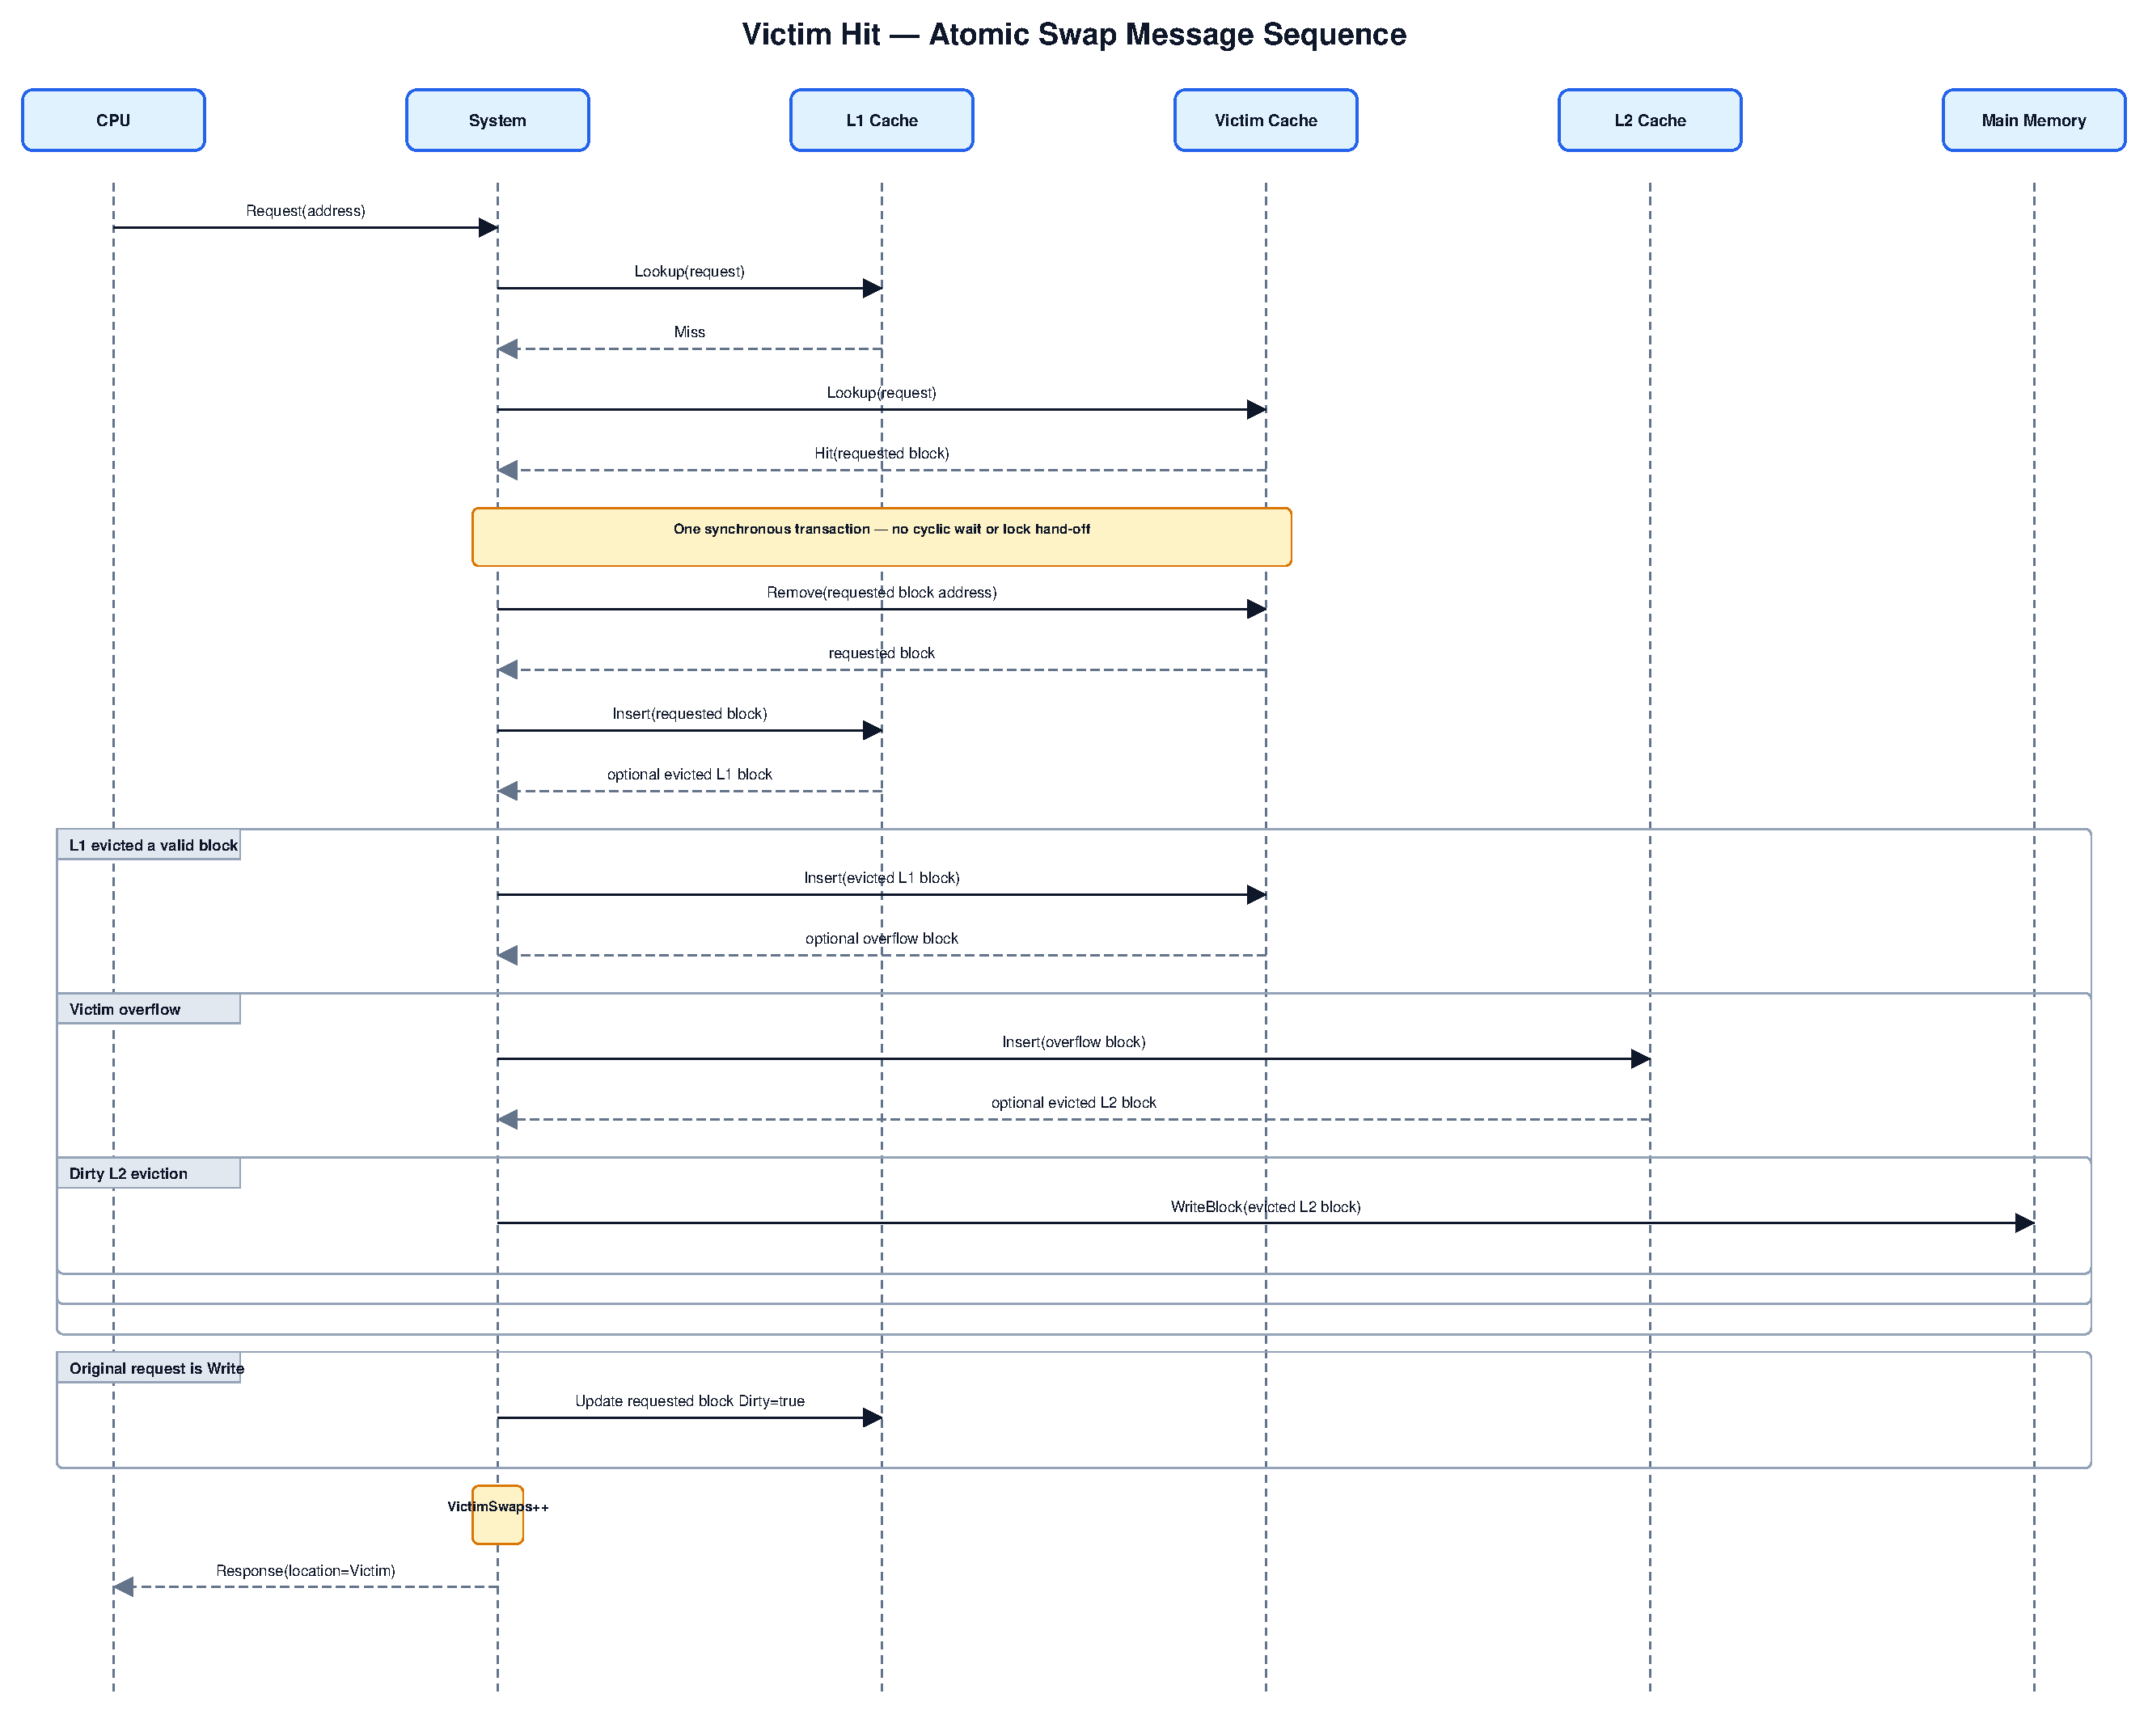
\includegraphics[width=.92\textwidth,height=.68\textheight,keepaspectratio]{images/07-victim-hit-atomic-swap-sequence.pdf}
\caption{توالی منطقی و اتمیک جابه‌جایی میان \lr{L1} و حافظه قربانی داخل \lr{System.Access}}
\label{fig:victim-swap-seq}
\end{figure}

\subsection{مدیریت جابه‌جایی بدون بن‌بست}
\label{subsec:swap-deadlock}

در مدل فعلی، درخواست‌ها به‌صورت سری پردازش می‌شوند و تابع \lr{System.Access} تمام تغییرات مربوط به یک درخواست را انجام می‌دهد. جابه‌جایی حافظه قربانی با ترتیب زیر انجام می‌شود:

\begin{enumerate}
\item بلوک درخواستی با \lr{Remove} از حافظه قربانی خارج و یک مدخل خالی ایجاد می‌شود؛
\item بلوک درخواستی در \lr{L1} نصب می‌شود و بلوک قبلی خط، در صورت معتبر بودن، دریافت می‌شود؛
\item بلوک اخراجی \lr{L1} در همان مدخل آزاد حافظه قربانی قرار می‌گیرد؛
\item پس از تکمیل جابه‌جایی، پاسخ پردازنده ساخته می‌شود.
\end{enumerate}

چون پردازش سری است و مدخل لازم پیش از نصب بلوک در \lr{L1} آزاد می‌شود، انتظار چرخه‌ای و سرریز هنگام جابه‌جایی رخ نمی‌دهد. در درج عادی نیز اگر حافظه قربانی پر باشد، بلوک جایگزین‌شده پس از پایان تغییر محلی به \lr{L2} فرستاده می‌شود.

در مسیر رویدادمحور فعلی آکیتا همین ترتیب حفظ شده است. راننده فقط یک درخواست معوق دارد و اجراکننده نیز با فیلد \lr{busy} از هم‌پوشانی جلوگیری می‌کند. پس از تحویل \lr{accessRequestMsg}، کل تغییر حالت یک درخواست در یک فراخوانی \lr{System.Access} انجام می‌شود؛ سپس \lr{completeAccessEvent} زمان‌بندی می‌گردد. بنابراین در مدل سازگاری فعلی نیازی به رزرو مستقل خط‌ها یا قفل‌گذاری میان چند درخواست هم‌زمان وجود ندارد.

\subsection{یکپارچه‌سازی با شبیه‌ساز آکیتا}

در این معماری، ارتباط با شبیه‌ساز آکیتا (نسخه 4.9.0) از طریق یک آداپتور پیاده‌سازی شده است. برای اجرای هر آزمایش، اجزای اصلی شامل موتور سریال (\lr{sim.NewSerialEngine})، تولیدکننده درخواست (\lr{RequestDriver}) و اجراکننده سلسله‌مراتب (\lr{HierarchyExecutor}) مقداردهی می‌شوند. ارتباطات از طریق پورت‌های ورودی/خروجی و تبادل پیام‌های استاندارد آکیتا (\lr{accessRequestMsg} و \lr{accessResponseMsg}) صورت می‌گیرد. درخواست‌ها توسط تولیدکننده به اجراکننده ارسال شده و نتایج پس از محاسبه تأخیر معادل، با استفاده از مکانیزم زمان‌بندی آکیتا (\lr{NCyclesLater}) و در قالب رویدادهای تکمیل (\lr{completeAccessEvent}) به سیستم بازگردانده می‌شوند.

\section{بخش‌های اصلی کد}

\subsection{پیکربندی و اعتبارسنجی}

فایل \lr{internal/config/config.go} پارامترهای معماری، توپولوژی، سیاست جایگزینی و تأخیرها را نگهداری می‌کند. توابع \lr{UsesL1}، \lr{UsesL2} و \lr{UsesVictim} مسیر فعال را از توپولوژی استخراج می‌کنند. اعتبارسنجی‌ها تضمین می‌کنند که ظرفیت‌ها بر اندازه بلوک بخش‌پذیر باشند، \lr{L1} مستقیم‌نگاشت باقی بماند و اندازه \lr{L2} با درجه انجمنی آن سازگار باشد.

\begin{latin}
\begin{lstlisting}[caption={\lr{Default hierarchy configuration}},label={lst:config}]
func Default() Config {
    return Config{
        Topology:            TopologyFull,
        BlockSizeBytes:      64,
        L1SizeBytes:         4 * 1024,
        L1Associativity:     1,
        VictimEntries:       8,
        VictimEnabled:       true,
        VictimPolicy:        ReplacementFIFO,
        L2SizeBytes:         64 * 1024,
        L2Associativity:     8,
        L1HitLatencyCycles:  1,
        VictimLatencyCycles: 2,
        L2LatencyCycles:     12,
        MemoryLatencyCycles: 100,
    }
}
\end{lstlisting}
\end{latin}

\subsection{حافظه نهان مستقیم‌نگاشت سطح اول}

ساختار \lr{L1} یک آرایه ۶۴ عضوی از بلوک‌ها نگهداری می‌کند. تابع \lr{decode} اندیس و برچسب را به شکل زیر محاسبه می‌کند:

\begin{latin}
\begin{lstlisting}[caption={\lr{L1 index and tag decoding}}]
func (c *L1) decode(blockAddress uint64) (index int, tag uint64) {
    numLines := uint64(len(c.lines))
    return int(blockAddress % numLines), blockAddress / numLines
}
\end{lstlisting}
\end{latin}

در صورت اصابت، مقدار \lr{LastUsed} به‌روزرسانی می‌شود. هنگام درج، اگر همان بلوک در خط موجود باشد فقط وضعیت آن تغییر می‌کند؛ در غیر این صورت بلوک قبلی به لایه سیستم بازگردانده می‌شود تا به حافظه قربانی یا \lr{L2} برود. \lr{L1} مستقیماً سطح پایین‌تری را فراخوانی نمی‌کند؛ در نتیجه آزمون واحد و اتصال آن به شبیه‌ساز ساده‌تر است.

\subsection{حافظه قربانی و سیاست‌های جایگزینی}

حافظه قربانی برای هر جست‌وجو هر هشت مدخل را بررسی می‌کند و در نتیجه تمام‌انجمنی است. در \lr{FIFO} بلوک با کمترین \lr{Inserted} و در \lr{LRU} بلوک با کمترین \lr{LastUsed} انتخاب می‌شود:

\begin{latin}
\begin{lstlisting}[caption={\lr{FIFO and LRU victim selection}}]
switch c.cfg.NormalizedVictimPolicy() {
case config.ReplacementLRU:
    // choose minimum LastUsed
    ...
default:
    // choose minimum Inserted
    ...
}
\end{lstlisting}
\end{latin}

برای حفظ تفاوت واقعی دو سیاست، زمان آخرین استفاده بلوک در \lr{L1} هنگام ورود به حافظه قربانی نگه داشته می‌شود. مقدار ساعت محلی فقط زمانی جایگزین می‌شود که \lr{LastUsed} صفر باشد. یک آزمون واحد نیز بررسی می‌کند که \lr{LRU} بلوک اخیراً استفاده‌شده را، حتی اگر زودتر وارد شده باشد، حفظ کند.

\subsection{حافظه نهان سطح دوم}

\lr{L2} دارای ۱۲۸ مجموعه و هشت راه در هر مجموعه است. اندیس مجموعه از باقیمانده تقسیم آدرس بلوک بر ۱۲۸ به دست می‌آید و برچسب خارج‌قسمت آن است. در هر مجموعه ابتدا راه خالی با شماره کمتر پر می‌شود و در صورت پر بودن مجموعه، بلوکی که قدیمی‌ترین \lr{Inserted} را دارد اخراج می‌شود. اصابت‌های \lr{L2} ترتیب \lr{FIFO} را تغییر نمی‌دهند.

\subsection{هماهنگ‌کننده سیستم و مسیر درخواست}

فایل \lr{internal/system/system.go} منطق کل سلسله‌مراتب را در تابع \lr{Access} متمرکز کرده است. ترتیب بررسی به صورت زیر است:

\begin{equation}
\mathrm{L1}\;\longrightarrow\;\mathrm{Victim}\;\longrightarrow\;\mathrm{L2}\;\longrightarrow\;\mathrm{MainMemory}.
\end{equation}

در هر مرحله تأخیر متناظر به تأخیر تجمعی درخواست افزوده می‌شود. هنگام اصابت، پاسخ با محل مربوطه ساخته شده و شمارنده مناسب افزایش می‌یابد. تابع \lr{installL1} اخراج \lr{L1} را به حافظه قربانی و در معماری پایه به \lr{L2} هدایت می‌کند. تابع \lr{forwardEviction} نیز سرریز حافظه قربانی را به \lr{L2} منتقل می‌کند.

\begin{latin}
\begin{lstlisting}[caption={\lr{Simplified System.Access control path}}]
if L1 hit {
    return L1 response
}
if Victim enabled && Victim hit {
    move requested block to L1
    move L1 eviction to Victim
    return Victim response
}
if L2 hit {
    install block in L1
    return L2 response
}
read block from memory
install in L2 and L1
return memory response
\end{lstlisting}
\end{latin}

\subsection{آداپتور و چرخه اجرای رویدادهای آکیتا}

برنامه فرمان، تابع \lr{System.Access} را مستقیماً فراخوانی نمی‌کند؛ آداپتور درخواست‌های مدل را به اجرای رویدادمحور آکیتا متصل می‌کند. تابع \lr{Adapter.Build} پیش از اجرا، وجود سیستم و معتبر بودن پیکربندی سلسله‌مراتب را کنترل می‌کند. تابع \lr{Adapter.Run} سپس برای همان آزمایش یک موتور تازه می‌سازد تا هیچ زمان، پیام یا رویدادی از اجرای قبلی باقی نماند.

\paragraph{ساخت گراف اجرا.}
سه شیء اصلی در آغاز ساخته می‌شوند: موتور سریال، راننده درخواست و اجراکننده سلسله‌مراتب. جزئیات زنجیره سازنده اتصال مستقیم در قطعه‌کد زیر با سه‌نقطه خلاصه شده است؛ در کد واقعی، همین اتصال با موتور و فرکانس یک گیگاهرتز ساخته می‌شود.

\begin{latin}
\begin{lstlisting}[caption={\lr{Core steps of Akita graph construction}}]
engine := sim.NewSerialEngine()
driver := newRequestDriver(engine, a.Requests)
hierarchy := newHierarchyExecutor(
    engine, simulationFrequency, a.System)
connection := directconnection.MakeBuilder().
    ...
    Build("MemoryHierarchyConnection")
connection.PlugIn(driver.Port)
connection.PlugIn(hierarchy.Port)
driver.Destination = hierarchy.Port.AsRemote()
driver.Start()
\end{lstlisting}
\end{latin}

هر مولفه یک پورت با ظرفیت ورودی و خروجی یک دارد. اتصال مستقیم هر دو پورت را عضو یک مسیر انتقال می‌کند و مقصد راننده برابر پورت دوردست اجراکننده قرار می‌گیرد. فراخوانی \lr{Start} یک رویداد در زمان صفر می‌سازد؛ بنابراین نخستین درخواست نیز مانند سایر کارها از صف رویداد موتور آغاز می‌شود، نه از یک فراخوانی مستقیم بیرون موتور.

\paragraph{زمان‌بندی پاسخ.}
اجراکننده پس از دریافت پیام، دقیقاً یک بار \lr{System.Access} را فراخوانی می‌کند. این تابع محل پاسخ‌گویی، تغییرات لازم در کش‌ها و تأخیر سرویس را تعیین می‌کند. اجراکننده پاسخ را همان لحظه ارسال نمی‌کند؛ تعداد چرخه‌های پاسخ با \lr{NCyclesLater} به زمان شبیه‌سازی تبدیل می‌شود و یک رویداد تکمیل در آن زمان ثبت می‌گردد. جزئیات ساخت پیام پاسخ در قطعه‌کد خلاصه شده است:

\begin{latin}
\begin{lstlisting}[caption={\lr{Core of response-completion scheduling}}]
response := e.System.Access(request.Request)
completionTime := e.Frequency.NCyclesLater(
    int(response.LatencyCycles), e.Engine.CurrentTime())
e.Engine.Schedule(&completeAccessEvent{...})
\end{lstlisting}
\end{latin}

تا پیش از اجرای \lr{completeAccessEvent}، پاسخ برای راننده قابل مشاهده نیست و اجراکننده با فیلد \lr{busy} درخواست هم‌پوشان را نمی‌پذیرد. هنگام اجرای رویداد، پیام پاسخ از پورت اجراکننده فرستاده می‌شود و اجراکننده آزاد می‌گردد. پس زمان سرویس محاسبه‌شده واقعاً در ترتیب زمانی آکیتا اثر می‌گذارد، هرچند منطق جست‌وجو و جایگزینی داخل \lr{System.Access} همگام باقی می‌ماند.

\paragraph{کنترل جریان و پایان اجرا.}
راننده در هر لحظه فقط یک درخواست معوق نگه می‌دارد. پس از دریافت پاسخ، هم شناسه \lr{RspTo} آکیتا و هم \lr{RequestID} مدل پروژه را کنترل می‌کند تا پاسخ اشتباه یا خارج از ترتیب ثبت نشود. فقط پس از موفقیت این دو بررسی، پاسخ ذخیره و درخواست بعدی فرستاده می‌شود. پس از آخرین پاسخ، رویداد تازه‌ای ساخته نمی‌شود؛ صف موتور تخلیه می‌گردد و \lr{engine.Run} بازمی‌گردد. این ترتیب، اجرای واقعی قابلیت‌های پیام‌رسانی و زمان‌بندی آکیتا را با رفتار قطعی و سری مدل مرجع سازگار نگه می‌دارد.

\subsection{شمارنده‌ها، \lr{AMAT} و خروجی \lr{CSV}}

ساختار \lr{metrics.Stats} تعداد کل درخواست‌ها، اصابت و عدم اصابت هر سطح، خواندن و نوشتن \lr{L2}، مراجعه به حافظه اصلی، تعداد جابه‌جایی و چرخه کل را ثبت می‌کند. نرخ‌ها به صورت شرطی محاسبه می‌شوند؛ برای مثال نرخ اصابت حافظه قربانی بر تعداد عدم اصابت‌های \lr{L1} تقسیم می‌شود و نرخ اصابت \lr{L2} بر تعداد درخواست‌هایی که واقعاً به \lr{L2} رسیده‌اند.

تست‌بنچ برای هر سناریو و توپولوژی یک سیستم و یک آداپتور تازه می‌سازد؛ خود \lr{Adapter.Run} نیز موتور سریال، مولفه‌ها، پورت‌ها و اتصال آکیتا را از نو ایجاد می‌کند. بنابراین وضعیت کش، شمارنده‌ها و صف رویداد از اجرای قبلی باقی نمی‌ماند. تنها پس از تکمیل همه پاسخ‌ها توسط موتور، خلاصه سیستم خوانده و خروجی \lr{results.csv} با ۱۹ ستون تولید می‌شود. علاوه بر حسابداری، بررسی می‌شود که جمع اصابت و عدم اصابت‌ها با تعداد درخواست‌ها سازگار باشد، مجموع تأخیر پاسخ‌ها با چرخه کل برابر باشد و رفتار مورد انتظار هر برنامه محک رخ دهد.

\section{منطق تست‌بنچ، نتایج و تحلیل کارایی}

\subsection{روش اجرای مقایسه}

هر چهار الگو روی سه توپولوژی \Arch{l1-l2}، \Arch{full-fifo} و \Arch{full-lru} اجرا می‌شوند. تست‌بنچ برای هر حالت یک سیستم، آداپتور و موتور آکیتای تازه می‌سازد؛ بنابراین هر ردیف \lr{CSV} حاصل اجرای مستقل و کامل موتور با کش‌های سرد و صف رویداد خالی است. اندازه‌ها و تأخیرها نیز در همه توپولوژی‌ها ثابت می‌مانند.

دستور اصلی تولید داده‌ها عبارت است از:

\begin{latin}
\begin{lstlisting}[language={},numbers=none]
go run ./cmd/testbench -csv results.csv
\end{lstlisting}
\end{latin}

فایل \Arch{results.csv} شامل ۲۰ ردیف حاصل از چهار الگو و پنج معماری است. هر ردیف پس از بازگشت موفق \lr{Adapter.Run} و تطبیق تعداد پاسخ‌های آکیتا با تعداد درخواست‌ها نوشته می‌شود. گزارش فقط ۱۲ ردیف مربوط به سه توپولوژی مورد مقایسه را استفاده می‌کند. تابع \lr{ValidateResults} نیز برای ماتریس کامل، ۱۷۹ کنترل حسابداری و رفتاری تعریف می‌کند.

\subsection{الگوی تکراری: سنجش گرم‌شدن \lr{L1} (\lr{repeated})}

در این الگو، یک آدرس ۳۲ بار خوانده می‌شود. نخستین دسترسی در \lr{L1} عدم اصابت دارد و ۳۱ دسترسی بعدی اصابت می‌کنند. هر سه توپولوژی همین الگو را ثبت می‌کنند، اما معماری پایه ۱۴۴ چرخه و دو معماری کامل ۱۴۶ چرخه زمان می‌برند. اختلاف دو چرخه، هزینه یک بررسی ناموفق حافظه قربانی در دسترسی نخست است.

\subsection{الگوی ترتیبی: حرکت کلمه‌به‌کلمه (\lr{sequential})}

الگوی ترتیبی ۳۲ کلمه چهار بایتی را با آدرس‌های زیر می‌خواند:

\begin{equation}
0,4,8,\ldots,124.
\end{equation}

هر بلوک ۶۴ بایتی شامل ۱۶ کلمه است؛ پس این الگو دو بلوک را فراخوانی می‌کند. نخستین کلمه هر بلوک عدم اصابت و ۱۵ کلمه بعدی اصابت \lr{L1} هستند. در نتیجه هر سه توپولوژی ۳۰ اصابت و دو عدم اصابت دارند. زمان اجرا در معماری پایه ۲۵۶ و در دو معماری کامل ۲۶۰ چرخه است؛ چهار چرخه اختلاف از دو بررسی ناموفق حافظه قربانی ناشی می‌شود.

\subsection{الگوی برخوردی: مشاهده عملی نقص برخورد (\lr{conflict})}
\label{subsec:conflict-test}

در این الگو، چهار بلوک با فاصله ۴۰۹۶ بایت، برابر ظرفیت \lr{L1}، هشت بار تکرار می‌شوند. شماره بلوک‌ها ۰، ۶۴، ۱۲۸ و ۱۹۲ است و هر چهار مورد در اندیس صفر \lr{L1} قرار می‌گیرند. در نتیجه تمام ۳۲ دسترسی در \lr{L1} عدم اصابت دارند.

در معماری پایه، چهار دسترسی نخست از حافظه اصلی و ۲۸ دسترسی بعدی از \lr{L2} پاسخ داده می‌شوند. بنابراین ۳۲ درخواست خواندن \lr{L2}، ۲۸ اصابت \lr{L2} و ۴ مراجعه حافظه ثبت می‌شود. در معماری کامل، پس از چهار عدم اصابت اولیه، یک بلوک در \lr{L1} و سه بلوک در حافظه قربانی باقی می‌مانند. ۲۸ دسترسی بعدی همگی اصابت حافظه قربانی و جابه‌جایی هستند؛ از این رو فقط چهار درخواست به \lr{L2} می‌رسد.

نتیجه عددی این تغییر عبارت است از:

\begin{itemize}
\item کاهش خواندن‌های \lr{L2} از ۳۲ به ۴، برابر \درصد{87.5}؛
\item کاهش چرخه کل از ۸۱۶ به ۵۴۴، برابر \درصد{33.33}؛
\item کاهش میانگین زمان دسترسی از \lr{25.5} به ۱۷ چرخه؛
\item نرخ اصابت حافظه قربانی برابر \درصد{87.5} و ۲۸ جابه‌جایی.
\end{itemize}

در این الگو، چهار بلوک به‌طور کامل در ترکیب یک خط \lr{L1} و سه مدخل حافظه قربانی جا می‌شوند؛ بنابراین هیچ سرریزی رخ نمی‌دهد و \lr{FIFO} و \lr{LRU} خروجی یکسان دارند.

\subsection{الگوی ترکیبی: ارزیابی جامع سلسله‌مراتب و تفکیک \lr{FIFO} از \lr{LRU} (\lr{mixed})}

الگوی ترکیبی ۱۳۱۲ درخواست دارد و سه الگوی دسترسی را کنار هم قرار می‌دهد:

\begin{enumerate}
\item \مهم{ارزیابی سیاست جایگزینی (۱۲۱۶ درخواست)}: در هر دوره، ابتدا ۹ بلوک \lr{A0..A8} بارگذاری می‌شوند و برای جلوگیری از اخراج، بلوک‌های \lr{A0..A3} مجدداً خوانده می‌شوند تا اصطلاحاً «داغ» بمانند. سپس با ورود ۹ بلوک جدید و متعارض (\lr{B0..B8})، بلوک‌های قبلی به حافظه قربانی منتقل شده و رقابت بر سر جایگزینی ایجاد می‌شود. دسترسی مجدد به \lr{A0..A3} در این حالت، تفاوت عملکرد \lr{FIFO} و \lr{LRU} را به‌خوبی آشکار می‌کند.
\item \مهم{ارزیابی محلی بودن داده‌ها (۳۲ درخواست)}: یک آدرس یکسان ۳۲ بار متوالی خوانده می‌شود که منجر به ۳۱ اصابت در \lr{L1} می‌گردد.
\item \مهم{دسترسی مشترک به حافظه قربانی (۶۴ درخواست)}: چهار بلوک متعارض ۱۶ بار تکرار می‌شوند تا رفتار و نرخ اصابت حافظه قربانی تحت هر دو سیاست بررسی شود.
\end{enumerate}

هر سه توپولوژی در این الگو ۶۶۷ اصابت و ۶۴۵ عدم اصابت \lr{L1} دارند؛ تفاوت در محل پاسخ‌گویی به عدم اصابت‌هاست. \lr{FIFO} تعداد ۶۰ اصابت حافظه قربانی و ۵۸۵ خواندن \lr{L2} ثبت می‌کند، در حالی که این اعداد برای \lr{LRU} به‌ترتیب ۱۸۸ و ۴۵۷ هستند. در نتیجه \lr{LRU} تعداد ۱۲۸ مراجعه \lr{L2} را با اصابت حافظه قربانی جایگزین می‌کند.

چرخه کل \lr{l1-l2} برابر ۱۱۳۵۲، \lr{full-fifo} برابر ۱۱۹۲۲ و \lr{full-lru} برابر ۱۰۳۸۶ است. \lr{FIFO} با وجود کاهش ترافیک \lr{L2}، به دلیل نرخ پایین اصابت حافظه قربانی و پرداخت هزینه بررسی آن در بسیاری از عدم اصابت‌ها، \درصد{5.02} از معماری پایه کندتر است. \lr{LRU} نسبت به معماری پایه \درصد{8.51} و نسبت به \lr{FIFO} حدود \درصد{12.88} چرخه کمتری مصرف می‌کند.

\subsection{تحلیل \lr{AMAT}}
\label{subsec:amat}

در مدل پروژه، تأخیرهای افزایشی برابر $T_{L1}=1$، $T_{VC}=2$، $T_{L2}=12$ و $T_M=100$ چرخه هستند. با نرخ‌های شرطی، \lr{AMAT} معماری پایه به صورت زیر محاسبه می‌شود:

\begin{equation}
\mathrm{AMAT}_{base}=T_{L1}+MR_{L1}\left(T_{L2}+MR_{L2}T_M\right).
\label{eq:amat-base}
\end{equation}

برای معماری دارای حافظه قربانی داریم:

\begin{equation}
\mathrm{AMAT}_{VC}=T_{L1}+MR_{L1}\left(T_{VC}+MR_{VC}\left(T_{L2}+MR_{L2}T_M\right)\right).
\label{eq:amat-vc}
\end{equation}

از آنجا که راننده آکیتا فقط یک درخواست معوق نگه می‌دارد و درخواست‌ها را سری اجرا می‌کند، ستون \lr{average\_cycles} همان \lr{AMAT} تجربی مدل است. این ستون از مجموع \lr{LatencyCycles} پاسخ‌های تکمیل‌شده محاسبه می‌شود، نه از تیک‌های داخلی انتقال در اتصال مستقیم آکیتا. جدول \ref{tab:amat} مقادیر اندازه‌گیری‌شده را نشان می‌دهد.

\begin{table}[H]
\centering
\caption{\lr{AMAT} اندازه‌گیری‌شده بر حسب چرخه برای هر درخواست}
\label{tab:amat}
\begin{latin}
\begin{tabular}{lrrr}
\toprule
\lr{Workload} & \lr{L1-L2} & \lr{Full-FIFO} & \lr{Full-LRU} \\
\midrule
\lr{Repeated}   & 4.500 & 4.562 & 4.562 \\
\lr{Sequential} & 8.000 & 8.125 & 8.125 \\
\lr{Conflict}   & 25.500 & 17.000 & 17.000 \\
\lr{Mixed}      & 8.652 & 9.087 & 7.916 \\
\bottomrule
\end{tabular}
\end{latin}
\end{table}

برای نمونه، در الگوی برخوردی $MR_{L1}=1$ و در معماری پایه $MR_{L2}=4/32=0.125$ است؛ در نتیجه:

\begin{equation}
1+1\times(12+0.125\times100)=25.5.
\end{equation}

در معماری کامل، نرخ عدم اصابت حافظه قربانی نیز $4/32=0.125$ است و تمام این چهار درخواست در \lr{L2} عدم اصابت دارند؛ بنابراین:

\begin{equation}
1+1\times\left(2+0.125\times(12+100)\right)=17.
\end{equation}

\subsection{نتایج کمّی و نمودارهای مقایسه‌ای}
\label{subsec:quant-results}

شکل \ref{fig:avg-cycles} میانگین چرخه هر درخواست را نشان می‌دهد. حافظه قربانی در الگوهایی که برخورد ندارند، سربار اندکی ایجاد می‌کند؛ اما در الگوی \Arch{conflict} بهبود بزرگ و در الگوی \Arch{mixed}، سیاست \lr{LRU} بهبود معنادار ایجاد می‌کند.

\begin{figure}[H]
\centering
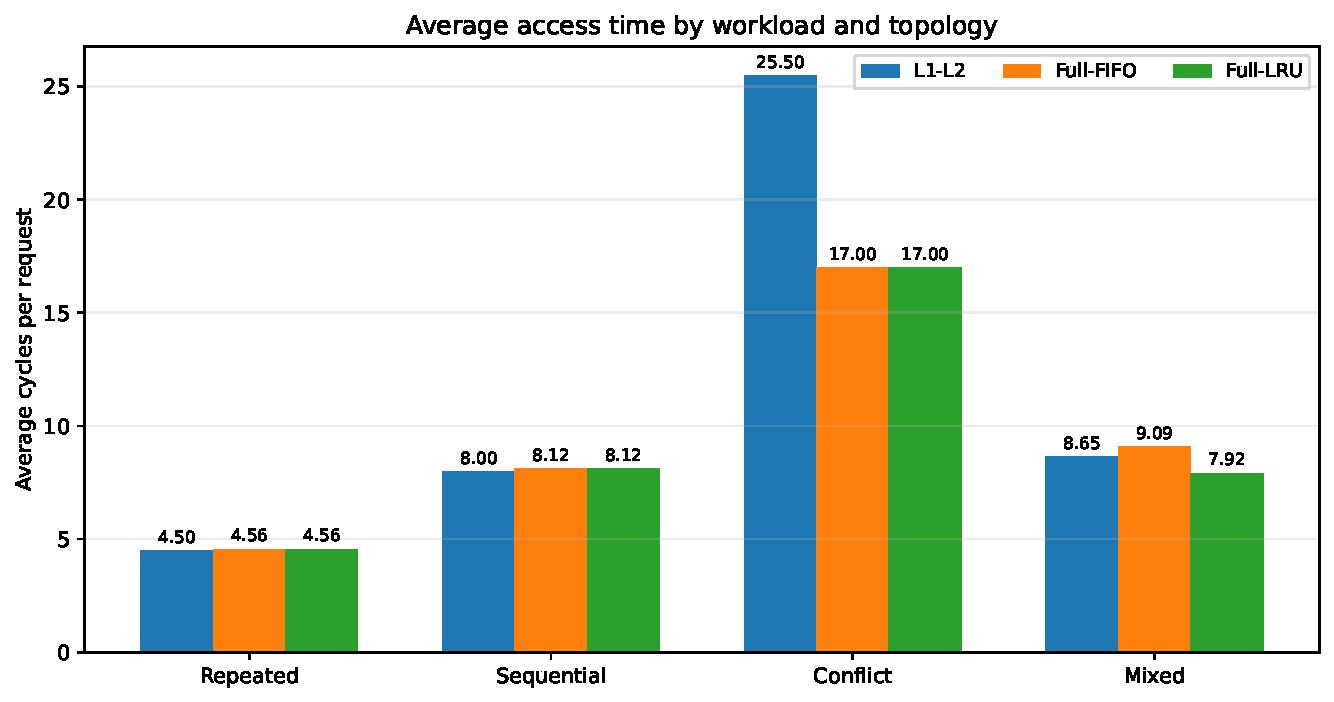
\includegraphics[width=.94\textwidth]{images/average_cycles_by_trace.pdf}
\caption{مقایسه میانگین چرخه هر درخواست در چهار برنامه محک}
\label{fig:avg-cycles}
\end{figure}

شکل \ref{fig:l2-traffic} تعداد خواندن \lr{L2} را نسبت به معماری پایه نرمال می‌کند. در الگوی \Arch{conflict} هر دو سیاست ترافیک را به \درصد{12.5} مقدار پایه می‌رسانند. در \Arch{mixed} مقدار متناظر برای \lr{FIFO} برابر \درصد{90.7} و برای \lr{LRU} برابر \درصد{70.9} است.

\begin{figure}[H]
\centering
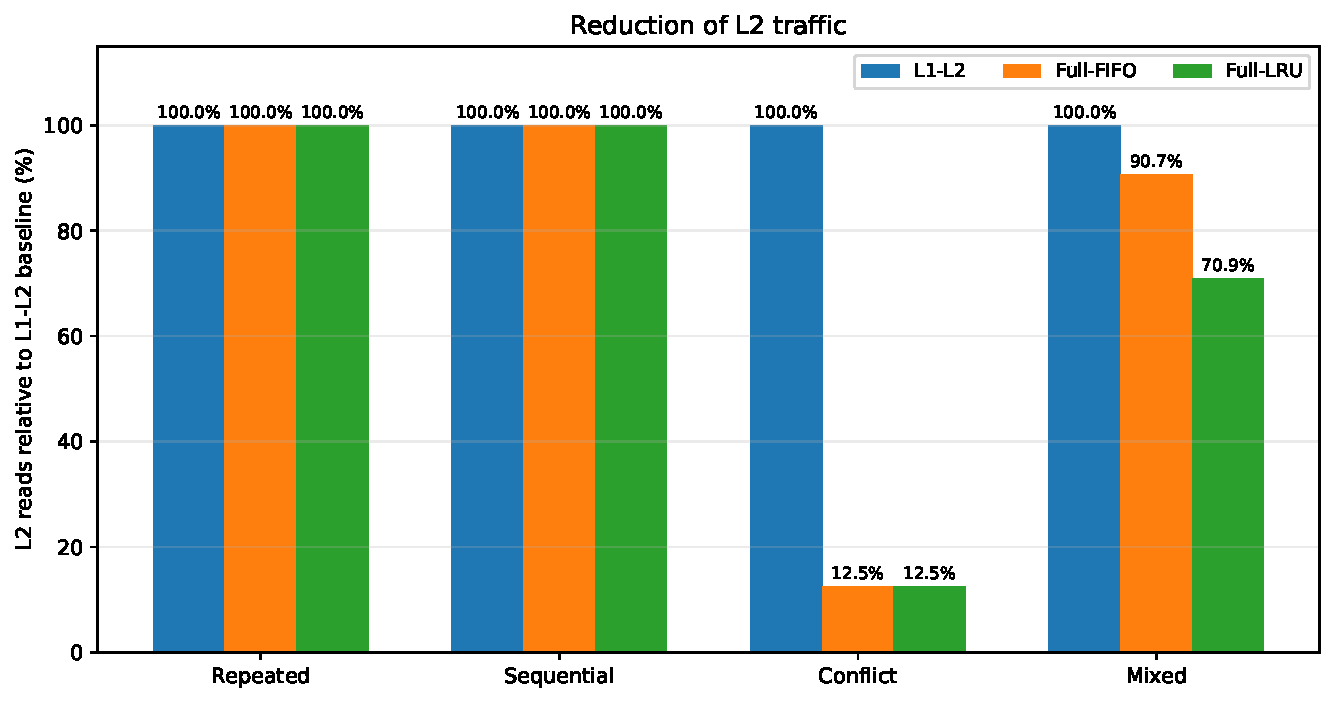
\includegraphics[width=.94\textwidth]{images/l2_reads_relative.pdf}
\caption{کاهش ترافیک خواندن \lr{L2} نسبت به توپولوژی پایه \lr{l1-l2}}
\label{fig:l2-traffic}
\end{figure}

شکل \ref{fig:vc-hit-rate} نشان می‌دهد که الگوی \Arch{conflict} برای هر دو سیاست نرخ اصابت \درصد{87.5} دارد، ولی در الگوی \Arch{mixed} نرخ اصابت \lr{LRU} از \درصد{9.30} در \lr{FIFO} به \درصد{29.15} افزایش می‌یابد.

\begin{figure}[H]
\centering
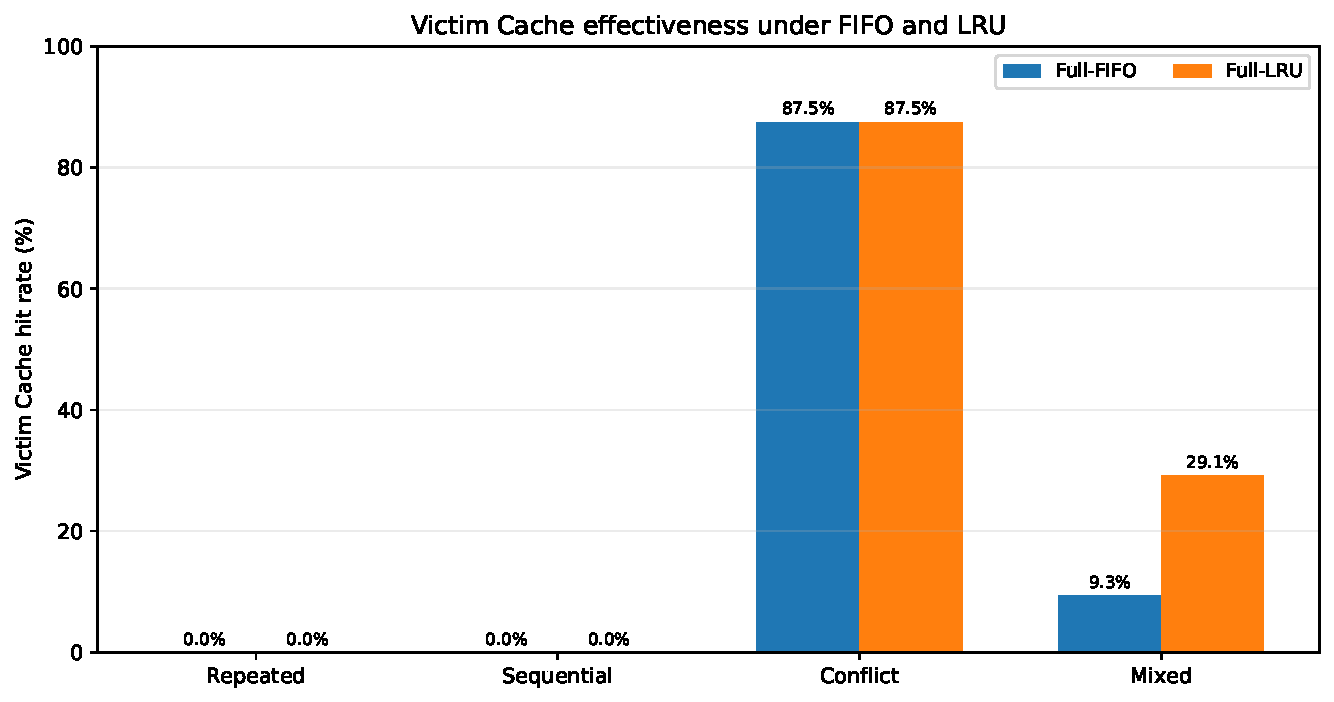
\includegraphics[width=.94\textwidth]{images/victim_hit_rate.pdf}
\caption{نرخ اصابت حافظه قربانی در سیاست‌های \lr{FIFO} و \lr{LRU}}
\label{fig:vc-hit-rate}
\end{figure}

شکل \ref{fig:cycle-relative} چرخه کل را نسبت به \Arch{l1-l2} نشان می‌دهد. خط صددرصد معماری پایه را مشخص می‌کند. کاهش مراجعه به \lr{L2} زمانی زمان اجرا را کم می‌کند که تعداد اصابت‌های حافظه قربانی برای جبران هزینه بررسی اضافی کافی باشد.

\begin{figure}[H]
\centering
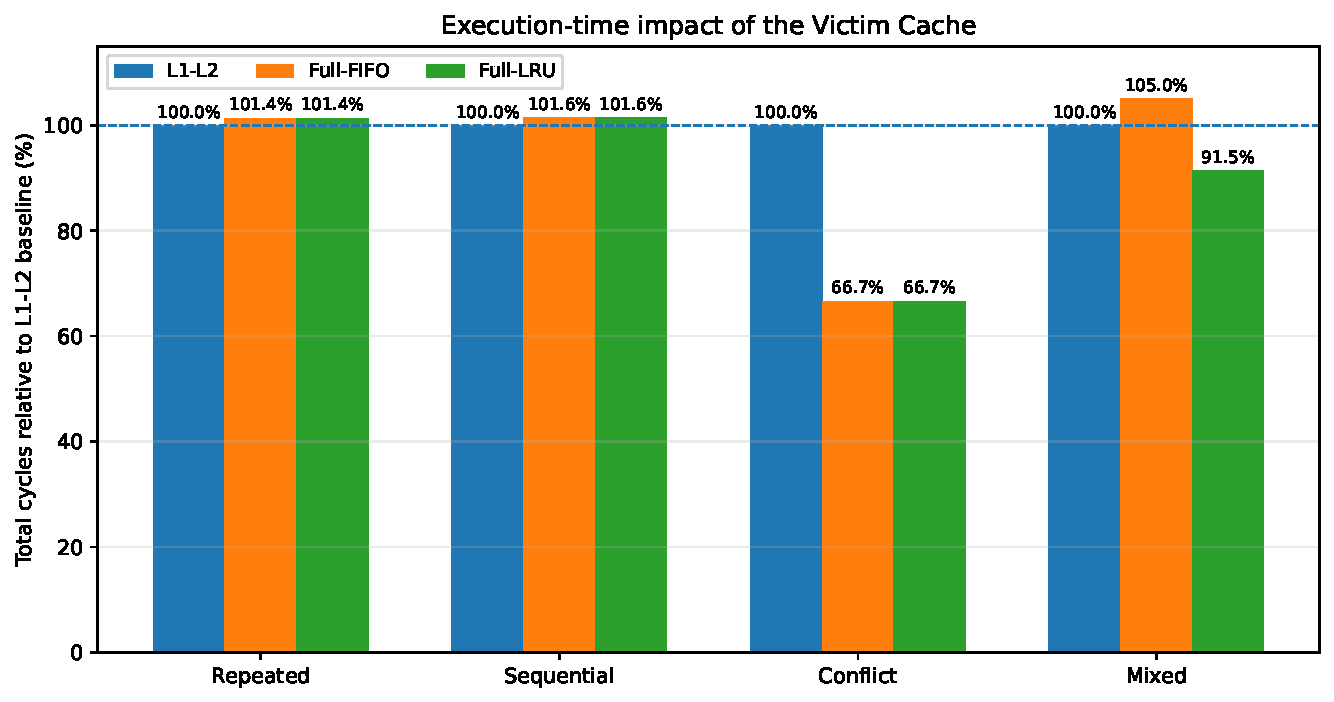
\includegraphics[width=.94\textwidth]{images/total_cycles_relative.pdf}
\caption{چرخه کل هر معماری نسبت به \lr{l1-l2}}
\label{fig:cycle-relative}
\end{figure}

شکل \ref{fig:mixed-policy} دو سیاست را در الگوی ترکیبی مقایسه می‌کند. \lr{LRU} با ۱۲۸ اصابت بیشتر در حافظه قربانی، دقیقاً ۱۲۸ خواندن \lr{L2} را حذف کرده است.

\begin{figure}[H]
\centering
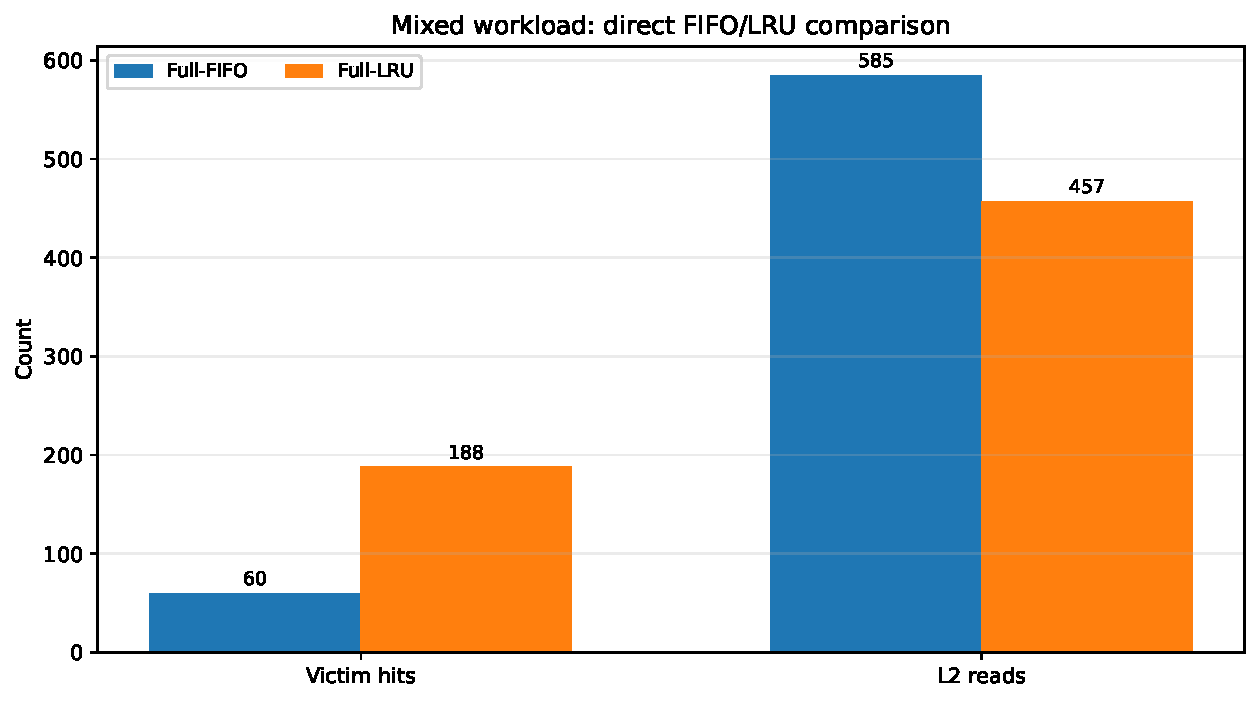
\includegraphics[width=.86\textwidth]{images/mixed_policy_counts.pdf}
\caption{مقایسه مستقیم \lr{FIFO} و \lr{LRU} در الگوی \lr{mixed}}
\label{fig:mixed-policy}
\end{figure}

\subsection{جمع‌بندی نتایج}

حافظه قربانی در الگوهای بدون برخورد فقط هزینه بررسی اضافی ایجاد می‌کند، اما در دسترسی‌های برخوردی می‌تواند بیشتر مراجعه‌های تکراری \lr{L2} را حذف کند. الگوی ترکیبی نیز اهمیت سیاست جایگزینی را نشان می‌دهد: \lr{LRU} با نگه‌داشتن بلوک‌های داغ، هم ترافیک \lr{L2} و هم زمان اجرا را کاهش می‌دهد؛ در حالی که \lr{FIFO} در این الگو حتی از معماری پایه کندتر است. 

\begin{appendix}

\section{خروجی کامل آزمایش‌ها و نحوه اجرا}

جدول‌های \ref{tab:timing-results} و \ref{tab:counter-results} دوازده ردیف استفاده‌شده از فایل \lr{results.csv} را نشان می‌دهند. ستون \lr{Avg.} برابر چرخه کل تقسیم بر تعداد درخواست‌ها است.

\clearpage
\begin{table}[H]
\centering
\caption{تعداد درخواست و زمان اجرای سه توپولوژی}
\label{tab:timing-results}
\begin{latin}
\small
\linespread{1}\selectfont
\renewcommand{\arraystretch}{1.55}
\setlength{\tabcolsep}{4pt}
\begin{tabular*}{0.99\textwidth}{@{\extracolsep{\fill}}llrrr@{}}
\toprule
\lr{Trace} & \lr{Architecture} & \lr{Req.} & \lr{Cycles} & \lr{Avg.} \\
\midrule
\lr{repeated} & \lr{l1-l2} & 32 & 144 & 4.500 \\
\lr{repeated} & \lr{full-fifo} & 32 & 146 & 4.562 \\
\lr{repeated} & \lr{full-lru} & 32 & 146 & 4.562 \\
\lr{sequential} & \lr{l1-l2} & 32 & 256 & 8.000 \\
\lr{sequential} & \lr{full-fifo} & 32 & 260 & 8.125 \\
\lr{sequential} & \lr{full-lru} & 32 & 260 & 8.125 \\
\lr{conflict} & \lr{l1-l2} & 32 & 816 & 25.500 \\
\lr{conflict} & \lr{full-fifo} & 32 & 544 & 17.000 \\
\lr{conflict} & \lr{full-lru} & 32 & 544 & 17.000 \\
\lr{mixed} & \lr{l1-l2} & 1312 & 11352 & 8.652 \\
\lr{mixed} & \lr{full-fifo} & 1312 & 11922 & 9.087 \\
\lr{mixed} & \lr{full-lru} & 1312 & 10386 & 7.916 \\
\bottomrule
\end{tabular*}
\end{latin}

\vspace{1.1cm}

\caption{شمارنده‌های سلسله‌مراتب حافظه در سه توپولوژی}
\label{tab:counter-results}
\begin{latin}
\small
\linespread{1}\selectfont
\renewcommand{\arraystretch}{1.55}
\setlength{\tabcolsep}{2.5pt}
\begin{tabular*}{0.99\textwidth}{@{\extracolsep{\fill}}llrrrrrrr@{}}
\toprule
\lr{Trace} & \lr{Architecture} & \lr{L1 H} & \lr{L1 M} & \lr{VC H} & \lr{VC M} & \lr{L2 Reads} & \lr{Mem.} & \lr{Swaps} \\
\midrule
\lr{repeated} & \lr{l1-l2} & 31 & 1 & 0 & 0 & 1 & 1 & 0 \\
\lr{repeated} & \lr{full-fifo} & 31 & 1 & 0 & 1 & 1 & 1 & 0 \\
\lr{repeated} & \lr{full-lru} & 31 & 1 & 0 & 1 & 1 & 1 & 0 \\
\lr{sequential} & \lr{l1-l2} & 30 & 2 & 0 & 0 & 2 & 2 & 0 \\
\lr{sequential} & \lr{full-fifo} & 30 & 2 & 0 & 2 & 2 & 2 & 0 \\
\lr{sequential} & \lr{full-lru} & 30 & 2 & 0 & 2 & 2 & 2 & 0 \\
\lr{conflict} & \lr{l1-l2} & 0 & 32 & 0 & 0 & 32 & 4 & 0 \\
\lr{conflict} & \lr{full-fifo} & 0 & 32 & 28 & 4 & 4 & 4 & 28 \\
\lr{conflict} & \lr{full-lru} & 0 & 32 & 28 & 4 & 4 & 4 & 28 \\
\lr{mixed} & \lr{l1-l2} & 667 & 645 & 0 & 0 & 645 & 23 & 0 \\
\lr{mixed} & \lr{full-fifo} & 667 & 645 & 60 & 585 & 585 & 23 & 60 \\
\lr{mixed} & \lr{full-lru} & 667 & 645 & 188 & 457 & 457 & 23 & 188 \\
\bottomrule
\end{tabular*}
\end{latin}
\end{table}

\clearpage
\subsection{دستورهای اجرای پروژه}

وابستگی پروژه آکیتا نسخه \lr{4.9.0} است و ماژول از \lr{Go 1.24} استفاده می‌کند. هیچ پرچم یا فرمان جداگانه‌ای برای فعال کردن آکیتا وجود ندارد: همه فرمان‌های عادی زیر به‌صورت پیش‌فرض از مسیر \lr{simadapter} و موتور آکیتا اجرا می‌شوند و قالب خروجی ترمینال و \lr{CSV} بدون تغییر باقی می‌ماند.

\begin{latin}
\begin{lstlisting}[language={},numbers=none]
# Run the complete deterministic suite and write CSV
go run ./cmd/testbench -csv results.csv

# Run one workload on the baseline
go run ./cmd/sim -topology l1-l2 -trace conflict

# Run mixed with FIFO
go run ./cmd/sim -topology full -trace mixed \
  -victim=true -victim-policy FIFO

# Run mixed with LRU
go run ./cmd/sim -topology full -trace mixed \
  -victim=true -victim-policy LRU

# Verification
go test ./...
go test -race ./...
go vet ./...
\end{lstlisting}
\end{latin}

\subsection{کنترل‌های خودکار مهم}

تست‌بنچ موارد زیر را به صورت خودکار بررسی می‌کند:

\begin{itemize}
\item برابر بودن تعداد درخواست، پاسخ و مجموع محل‌های پاسخ‌گویی؛
\item برابری مجموع اصابت و عدم اصابت \lr{L1} با تعداد درخواست‌ها؛
\item برابری مجموع اصابت و عدم اصابت حافظه قربانی با تعداد عدم اصابت‌های \lr{L1}؛
\item برابری اصابت و عدم اصابت \lr{L2} با تعداد خواندن‌های \lr{L2}؛
\item تطابق مجموع چرخه پاسخ‌ها با شمارنده چرخه کل؛
\item تولید دقیق ۳۰ اصابت و دو عدم اصابت در الگوی ترتیبی پیش‌فرض؛
\item کاهش خواندن \lr{L2} و چرخه در الگوی برخوردی؛
\item بیشتر بودن اصابت حافظه قربانی و کمتر بودن خواندن \lr{L2} و چرخه کل \lr{LRU} نسبت به \lr{FIFO} در الگوی ترکیبی.
\end{itemize}

علاوه بر کنترل‌های بالا، آزمون \Arch{internal/simadapter/adapter\_test.go} هر چهار الگو را روی پنج معماری اجرا می‌کند و پاسخ‌ها و تمام شمارنده‌های اجرای آکیتا را با \lr{System.Run} به‌عنوان مدل مرجع مقایسه می‌کند. این آزمون همچنین تکمیل موفق موتور، اجرای الگوی خالی، کپی شدن ورودی‌ها، ضرورت \lr{Build} و هویت مستقل نسخه کپی‌شده پیام‌ها را کنترل می‌کند.

\subsection{فایل‌های همراه گزارش}

فایل \lr{results-selected.csv} در ریشه بسته \lr{LaTeX} شامل همان ۱۲ ردیف استفاده‌شده در گزارش است. چهار نمودار ماشین حالت و توالی منطقی عملیات به صورت \lr{PDF} در پوشه \lr{images} قرار دارند و نسخه \lr{SVG} آن‌ها نیز در \lr{images/svg-source} نگهداری شده است. نمودارهای توالی، فراخوانی‌های داخلی \lr{System.Access} را نشان می‌دهند؛ مسیر پیام واقعی آکیتا همان راننده، اتصال مستقیم و اجراکننده‌ای است که در بخش پیاده‌سازی آکیتا تشریح شد.

\end{appendix}

\end{document}